\chapter{B\'{e}zier $\bar{B}$ projection}
\label{chp:chapter6}
\graphicspath{{figures/}{figures/chapter6/}}
\pgfplotsset{
  table/search path={{figures/chapter6/data},{data}},
}

In this chapter, we demonstrate how dual basis functions can be employed as the underlying local projection framework for a $\bar{B}$ approach to treat locking in isogeometric structural elements.

Numerical locking in structural finite elements includes geometric locking in thin curved structural members such as membrane and shear locking and also includes volumetric locking in incompressible and nearly incompressible elasticity. There is an immense body of literature on approaches to overcome locking in the finite element community and various approaches have emerged as dominant. These include reduced quadrature~\cite{malkus_mixed_1978,zienkiewicz_reduced_1971}, $\bar{B}$ projection methods~\cite{nagtegaal_numerically_1974,hughes_generalization_1980, NME:NME4328}, and mixed methods based on the Hu-Washizu variational principle~\cite{dolbow_volumetric_1999,kasper_mixed-enhanced_2000,hughes_variational_1986, NME:NME3048}. It is important to mention that, although ameliorated at high polynomial degrees, smooth splines in the context of IGA still exhibit locking behavior~\cite{echter_numerical_2010, bouclier_locking_2012}.

In IGA, there is a growing literature on the treatment of locking in structural elements. Leveraging higher-order smoothness, transverse shear locking can be eliminated at the theoretical level by employing Kirchhoff-Love~\cite{kiendl2009isogeometric, kiendl2015isogeometric} and hierarchic Reissner-Mindlin~\cite{oesterle_hierarchic_2017, oesterle_shear_2016,echter_hierarchic_2013} shell elements. Reduced quadrature schemes have been explored in~\cite{adam_improved_2014, adam_improved_2015, adam_selective_2015} as a way to alleviate transverse shear locking. The extension of $\bar{B}$ projection to the isogeometric setting was initiated in~\cite{elguedj:hal-00457010} for both elastic and plastic problems and was extended in~\cite{bouclier_efficient_2013} to include local projection techniques~\cite{mitchell_method_2011,govindjee_convergence_2012}.

In this chapter we introduce two methods that employ \Bezier dual basis to produce a localized approximation to the standard $\bar{B}$ method. The motivation behind these methods is the fact that $\bar{B}$ methods result in dense linear systems. The methods we introduce result in a sparse linear system irrespective of the choice of basis functions. We call these two methods the symmetric and non-symmetric \Bezier $\bar{B}$ projection methods, where the names indicate the symmetry of the resulting stiffness matrix. We show that both methods result in a sparse stiffness matrix and reduce locking. We also show that optimal convergence rates are achieved in the case of the non-symmetric method and near optimal convergence rates are achieved in the case of the symmetric method.  We also perform an inf-sup analysis of these methods.

\section{Geometric locking: Timoshenko beams}
\label{sec:timoshenkobeam}
To illustrate the use of \Bezier $\bar{B}$ projection to overcome geometric locking effects we study transverse shear locking in Timoshenko beams. The Timoshenko beam problem provides a simple one dimensional setting in which to describe B\'ezier $\bar{B}$ projection. Note however, that the approach can be directly generalized to more complex settings like spatial beams and shells and other geometric locking mechanisms like membrane locking. We consider a planar cantilevered Timoshenko beam as shown in Figure~\ref{fig:Timoshenko_beam_cross}. The strong form for this problem can be stated as
\begin{align}
  \begin{rcases}
    \begin{aligned}
      -s{GA}\gamma'          & =f(x)          \\
      -EI\kappa'-s{GA}\gamma & = 0            \\
      \kappa                 & = \phi'        \\
      \gamma                 & = \omega'-\phi
    \end{aligned}
  \end{rcases}
   & \text{ in $\Omega$} \\
  \begin{rcases}
    \begin{aligned}
      \omega & =0 \\
      \phi   & =0
    \end{aligned}
  \end{rcases}
   & \text{ at $x=0$}    \\
  \begin{rcases}
    \begin{aligned}
      s{AG}\gamma & = Q \\
      -EI\kappa   & = M
    \end{aligned}
  \end{rcases}
   & \text{ at $x=L$}
\end{align}
where $\gamma$ is the shear strain, $\kappa$ is the bending strain, $\omega$ is the vertical displacement, $\phi$ is the angle of rotation of the normal to the mid-plane of the beam, $f$ is the distributed transverse load, $Q$ is a point load, $M$ is the moment, $E$ is the Young's modulus, $G$ is the shear modulus, $A$ is the cross-sectional area, $I$ is the second moment of inertia of the beam cross-section, $s$ is the shear correction factor, normally set to $5/6$ for rectangular cross-sections, and $\Omega = (0,L)$. When $\omega$ and $\phi$ are interpolated by basis functions of the same order the finite element solution to this problem exhibits shear locking as the beam becomes slender.

\begin{figure}[ht]
  \centering
  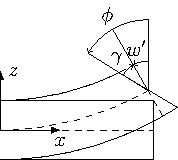
\includegraphics[width=0.25\linewidth]{timoshenko_beam_shape}
  \caption{Deformation of a Timoshenko beam. The normal rotates by the angle $\phi$, which is not equal to $w'$, due to shear deformation.}
  \label{fig:Timoshenko_beam_cross}
\end{figure}

\subsection{Symmetric \Bezier $\bar{B}$ projection}
\label{sec:symmetric-projection}
Locking is caused in Timoshenko beam problems when equal order interpolation is used for both midline displacements and rotations. To reduce the effects of locking for these problems the $\bar{B}$ method projects the shear strain, $\gamma$, onto a lower order function space. This process produces a projected shear strain, which we call $\bar{\gamma}$,  that is substituted into the weak form of the problem statement. In this section we use the \Bezier projection operator to compute an approximation of $\bar{\gamma}$, and refer to this approach as the symmetric \Bezier $\bar{B}$ projection method because the resulting stiffness matrix is symmetric.

\subsubsection{The weak form}

\sloppy Given the function spaces $\mathcal{S}(\Omega)=\{{\mathbf{u} \, \vert \, {\mathbf{u}\in{H^1(\Omega)\times{H^1(\Omega)}}},\mathbf{u}\vert_{\Gamma_{g}}=\mathbf{g}}\}$ and $\mathcal{V}(\Omega)=\{{\mathbf{w} \, \vert \, {\mathbf{w}\in{H^1(\Omega)\times{H^1(\Omega)}}}, \allowbreak \mathbf{w}\vert_{\Gamma_{g}}=\mathbf{0}}\}$ where $\mathbf{u}=\left\{{\omega,\phi}\right\}^T$, $\mathbf{w}=\left\{{\delta\omega,\delta\phi}\right\}^T$, $\mathbf{g}$ is the prescribed Dirichlet boundary condition, and $\Gamma_g$ is the Dirichlet boundary at $x=0$, the weak form of the problem can be stated as: find $\mathbf{u}\in{\mathcal{S}(\Omega)}$ such that for all $\mathbf{w}\in{\mathcal{V}(\Omega)}$
\begin{equation}
  {\int_{0}^L\kappa(\mathbf{w})EI\kappa(\mathbf{u}) + \bar{\gamma}(\mathbf{w})sGA\bar{\gamma}(\mathbf{u})} \, dx=\int_0^L\delta\omega f dx+\delta\omega(L)Q+\delta\phi(L)M.
\end{equation}

\subsubsection{Discretization}
We discretize $\omega$ and $\phi$ as
\begin{align}
  {\omega = \sum_A \omega_A N_A} \\
  {\phi = \sum_A \phi N_A}
\end{align}
where $N_A$ is a degree $p$ spline basis function and $\omega_A$ and $\phi_A$ are the corresponding control point values. The shear strain and bending strain can then be expressed as
\begin{align}
  \gamma & = \sum_A{\begin{bmatrix}N'_A & -N_A\end{bmatrix}\begin{bmatrix}\omega_A & \phi_A\end{bmatrix}^T} \\
  \kappa & = \sum_A\begin{bmatrix}0 & N'_A\end{bmatrix}\begin{bmatrix}\omega_A & \phi_A\end{bmatrix}^T
\end{align}
The shear strain $\bar{\gamma}$ is constructed by B\'{e}zier projection of the true shear strain $\gamma$ onto a lower degree space. In other words, we project from a $p^{th}$ degree spline space with $n$ basis functions $\mathbf{N}$ defined by the knot vector
\begin{align}
  \mathbf{\Xi}_{p}=\lbrace{\underbrace{0,0,\ldots,0}_\text{$p+1$ copies}},\mathbf{\Xi}_{int},{\underbrace{1,1,\ldots,1}_\text{$p+1$ copies}}\rbrace,
  \label{eq:origin_knot_vector}
\end{align}
onto a $p-1^{th}$ degree spline space with $\bar{n}$ basis functions $\bar{\mathbf{N}}$ defined by the knot vector
\begin{equation}
  \bar{\mathbf{\Xi}}_{p-1}=\lbrace{\underbrace{0,0,\ldots,0}_\text{$p$ copies}},\mathbf{\Xi}_{int},{\underbrace{1,1,\ldots,1}_\text{$p$ copies}}\rbrace
  \label{eq:projected_knot_vector}
\end{equation}
where the internal knots, denoted by $\mathbf{\Xi}_{int}$, are the same for both spaces. The projected shear strain $\bar{\gamma}$ can then be written as
\begin{align}
  \bar{\gamma} & = \sum_A \bar{\gamma}_A \bar{N}_A.
\end{align}
The control variables $\bar{\gamma}_A$ are simply
\begin{align}
  \bar{\gamma}_A = \int_{\Omega^A} \hat{\bar{N}}_A \gamma \, d\Omega = \langle \hat{\bar{N}}_A, \gamma \rangle_{\Omega^i}
\end{align}
where $\hat{\bar{N}}_A$ is a dual basis function for the spline space of degree $p-1$ computed from \eqref{eq:bezier-dual-basis}.

Localizing to the B\'{e}zier element we define the strain-displacement arrays in terms of element Bernstein basis functions of degree $p$ and $p-1$ as
\begin{align}
	\mathbf{B}_e^\kappa 
    	&= \begin{bmatrix} 0 & -{B^e_{0,p}}' & \cdots & 0 & -{B^e_{p,p}}' \end{bmatrix}, \\
    \mathbf{B}_e^\gamma
    	&= \begin{bmatrix} {B^e_{0,p}}' & -B^e_{0,p} & \cdots & {B^e_{p,p}}' & -B^e_{p,p} \end{bmatrix}, \\
    \bar{\mathbf{B}}_e
    	&= \begin{bmatrix} \bar{B}^e_{0,p-1} & \cdots & \bar{B}^e_{p-1,p-1} \end{bmatrix},
\end{align}
{where $B^e_{i,p}$ is the $i^{th}$ Bernstein basis function of order $p$}. We can then compute the element arrays as
\begin{align}
\mathbf{K}_e^b &= EI\mathbf{C}^e\langle{{\mathbf{B}_e^\kappa}^T,\mathbf{B}_e^\kappa}\rangle(\mathbf{C}^e)^T, \label{eq:symmetric_timoshenko}\\
\bar{\mathbf{M}}_e &= s{GA}\bar{\mathbf{C}}^e\langle{\bar{\mathbf{B}}_e^T,\bar{\mathbf{B}}_e}\rangle(\bar{\mathbf{C}}^e)^T, \\
{\hat{\mathbf{P}}_e} &= \langle{(\hat{\bar{\mathbf{N}}}^e)^T,\mathbf{B}^\gamma_e}\rangle(\mathbf{C}^e)^T \label{eq:P-hat-elem},
\end{align}
where $\mathbf{C}^e$ is the element extraction operator for the degree $p$ spline space, $\bar{\mathbf{C}}^e$ is the element extraction operator for the degree $p-1$ spline space, and $\hat{\bar{\mathbf{N}}}^e$ are the dual basis functions restricted to the element for the degree $p-1$ spline space. The global stiffness matrix can then be written as
\begin{align}
	\mathbf{K} = \mathbf{K}^b + \bar{\mathbf{K}}^s_S \label{eqn:symmetric_b_bar_timoshenko_stiffness}
\end{align}
where
\begin{align}
	\mathbf{K}^b &=\A_e\mathbf{K}_e^b,\label{eqn:bending_stiffness} \\
	\bar{\mathbf{K}}^s&={\hat{\mathbf{P}}}^T\bar{\mathbf{M}}{\hat{\mathbf{P}}}\label{eqn:shear_stiffness} \\
	{\hat{\mathbf{P}}} &=\A_e{\hat{\mathbf{P}}_e} \label{eq:P-hat-global}\\
    \bar{\mathbf{M}} &=\A_e\bar{\mathbf{M}}_e
\end{align}
and $\A$ is the standard finite element assembly operator \cite{Hug00}. We note that the assembly of $\bar{\mathbf{K}}^s$ requires the assembly of two intermediate matrices, $\bar{\mathbf{M}}$ and ${\hat{\mathbf{P}}}$. The computation of these matrices is needed because the product of two integrals over the entire domain can not be localized to the element level.

\subsection{Non-symmetric \Bezier $\bar{B}$ projection}
\label{sec:non-symmetric}

{Simo and Hughes \cite{Hug00} have shown that $\bar{B}$ formulations and mixed formulations are equivalent. However, the development of the symmetric \Bezier $\bar{B}$ projection method presented in Section~\ref{sec:symmetric-projection}, where we began by interpreting the $\bar{B}$ formulation as a strain projection method, lacks a connection to mixed formulations. In this section, we present a second method based on \Bezier projection in which we view the $\bar{B}$ formulation as a mixed formulation where, for the Timoshenko beam problem, the auxiliary variable is the shear stress. We use the \Bezier dual basis functions as the test functions for the auxiliary variable. Once the problem has been cast as a mixed formulation we then eliminate the auxiliary variable to get a purely displacement based formulation. This approach preserves convergence rates and all assembly routines for the stiffness matrix can be performed at the element level. However, it does not produce a symmetric stiffness matrix.}

\subsubsection{The weak form}
{In the mixed formulation for the Timoshencko beam problem the shear stress, $\tau=sGA\gamma$, is taken as a new independent variable. The weak form of the mixed formulation can then be stated as: find $\mathbf{u}\in{\mathcal{S}(\Omega)}$ and $\tau\in{L}^2(\Omega)$ such that for all $\mathbf{w}\in{\mathcal{V}(\Omega)}$ and $\delta\tau\in{L}^2(\Omega)$}
\begin{align}
    \int_{0}^L\kappa(\mathbf{w})EI\kappa(\mathbf{u}) + {\gamma}(\mathbf{w})\tau \, dx&= l\langle{\mathbf{w}}\rangle\\
    \int_{0}^L\delta\tau(sGA\gamma(\mathbf{u})-\tau) \, dx &= 0.
\end{align}
\subsubsection{Discretization}
{In the finite element formulation of the mixed problem, the discretization of $\mathbf{u}$ and $\mathbf{w}$ remain the same as before. The shear strain and its variation, however, are in $L^2(\Omega)$, so their finite element approximation can consist of functions with lower regularity, such as discontinuous polynomials. When the field $\mathbf{u}$ is discretized by $p^{th}$ degree spline basis functions defined by the knot vector given in \eqref{eq:origin_knot_vector}, we use the $p-1$ degree spline basis functions, defined by the knot vector given in \eqref{eq:projected_knot_vector}, to discretize the shear stress $\tau$ and the corresponding dual basis to discretize its variation $\delta\tau$. The discrete form of the shear stress and its variation are given by}
\begin{align}
    \tau&=\sum_A\tau_A\bar{N}_A \\
    \delta\tau&=\sum_A\delta\tau_A\hat{\bar{N}}_A.
\end{align}
{The stiffness matrix for the mixed form can then be written as}
\begin{equation}
   \mathbf{K}_{mix} =  
    \begin{bmatrix}
        \mathbf{K}^b & \mathbf{P}^T \\
        sGA\hat{\mathbf{P}} & -\mathbf{I}
    \end{bmatrix}
    \label{eq:mixed_timoshenko}
\end{equation}
{where}
\begin{equation}
    \mathbf{P}=\A_e\mathbf{P}_e,
\end{equation}
{and}
\begin{equation}
    \mathbf{P}_e=\bar{\mathbf{C}}^e\langle{\bar{\mathbf{B}}_e^T,\mathbf{B}^\gamma_e}\rangle(\mathbf{C}^e)^T.
\end{equation}
{ and $\hat{\mathbf{P}}$ is given in \eqref{eq:P-hat-elem} and \eqref{eq:P-hat-global}.
We can now eliminate the control variable of the shear stress from \eqref{eq:mixed_timoshenko} to get a pure displacement formulation where the stiffness matrix can be written as}
\begin{equation}
    \mathbf{K}=\mathbf{K}^b+\bar{\mathbf{K}}^s_{NS}, 
\end{equation}
where 
\begin{equation}
    \bar{\mathbf{K}}^s_{NS}=sGA\mathbf{P}^T\hat{\mathbf{P}}.
    \label{eq:nonsymmetric_timoshenko}
\end{equation}
{We can see that the use of different function spaces for the shear strain and its variation leads to a non-symmetric stiffness matrix.}

\paragraph{Remark} { As mentioned previously, the symmetric \Bezier $\bar{B}$ formulation is not consistent with a mixed formulation. To see this, we can recover the mixed formulation of \eqref{eqn:symmetric_b_bar_timoshenko_stiffness}, which is}
\begin{equation}
    \begin{bmatrix}
        \mathbf{K}^b & \hat{\mathbf{P}}^T \\
        sGA\hat{\mathbf{P}} & -\bar{\mathbf{M}}^{-1}
    \end{bmatrix},
\end{equation}
{where both the shear stress and its variation are discretized by the dual basis functions. However, for the inner product of dual basis functions we have}
\begin{equation}
    \langle{\hat{\bar{N}}_i,\hat{\bar{N}}_j}\rangle\neq{\bar{\mathbf{M}}^{-1}_{ij}},
\end{equation}
{which shows the inconsistency between the symmetric \Bezier $\bar{B}$ formulation and the mixed formulation.}

\subsection{Bandwidth of the stiffness matrix}
A global $\bar{B}$ method that utilizes a global $L^2$ projection results in a dense stiffness matrix. The B\'ezier $\bar{B}$ {methods}, on the other hand, {produce} sparse stiffness matrices. However, the coupling of the local dual basis functions does increase the bandwidth slightly. This is illustrated in Figure~\ref{fig:stiffness_matrix}, which shows the structure of the stiffness matrix for the Timoshenko beam problem using the second order basis functions of maximal smoothness for a displacement-based method (Figure~\ref{fig:stiffness_matrix}a), global $\bar{B}$ method (Figure~\ref{fig:stiffness_matrix}b), symmetric B\'ezier $\bar{B}$ method (Figure~\ref{fig:stiffness_matrix}c) and non-symmetric \Bezier $\bar{B}$ method (Figure~\ref{fig:stiffness_matrix}d). The blank cells indicate zero terms in the matrix while colored cells show the location of nonzero terms.
\begin{figure}[!htb]
    \centering
    \begin{subfigure}[b]{0.47\linewidth}        %% or \columnwidth
        \centering
        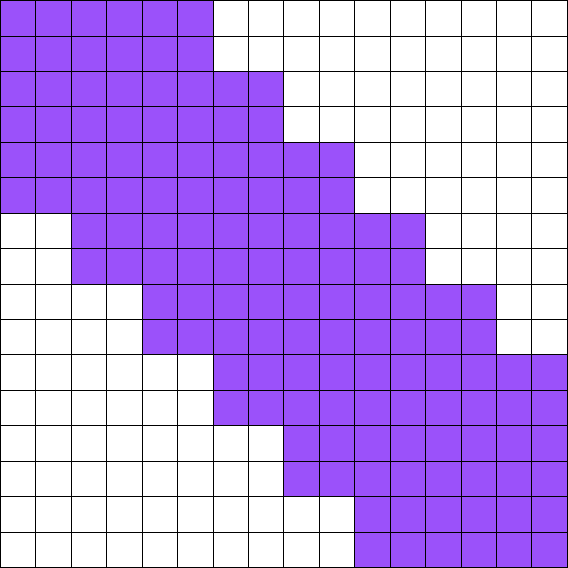
\includegraphics[width=\linewidth]{Global}
        \caption{Standard}
        %\label{}
    \end{subfigure}
    \begin{subfigure}[b]{0.47\linewidth}        %% or \columnwidth
        \centering
        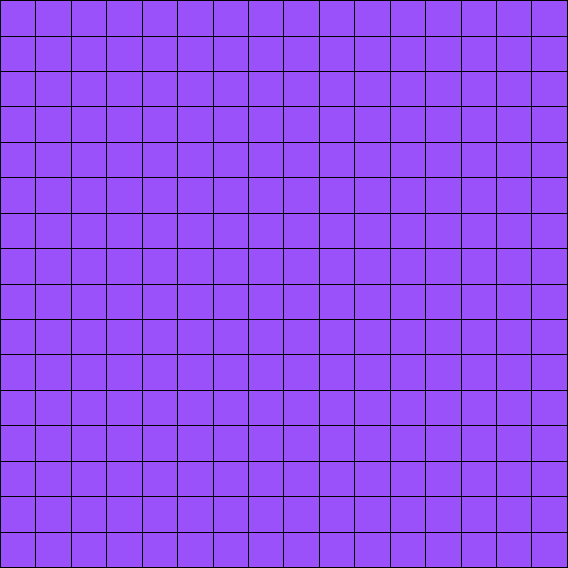
\includegraphics[width=\linewidth]{B_extraction}
        \caption{Global $\bar{B}$}
        %\label{}
    \end{subfigure}
    \begin{subfigure}[b]{0.47\linewidth}        %% or \columnwidth
        \centering
        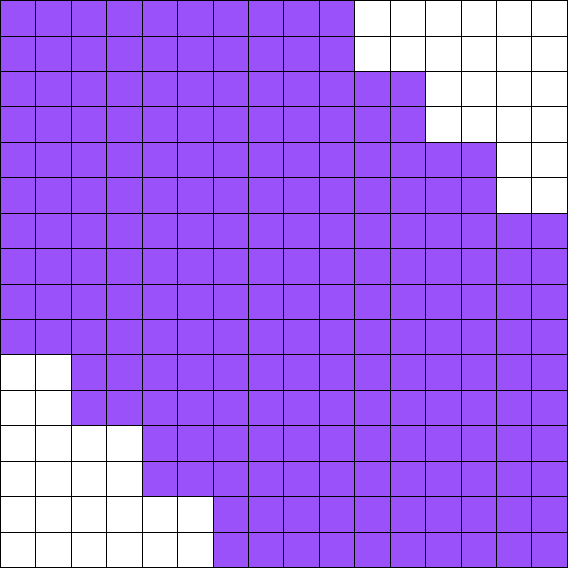
\includegraphics[width=\linewidth]{LB_extraction}
        \caption{Symmetric B\'ezier $\bar{B}$}
        %\label{}
    \end{subfigure}
    \begin{subfigure}[b]{0.47\linewidth}        %% or \columnwidth
        \centering
        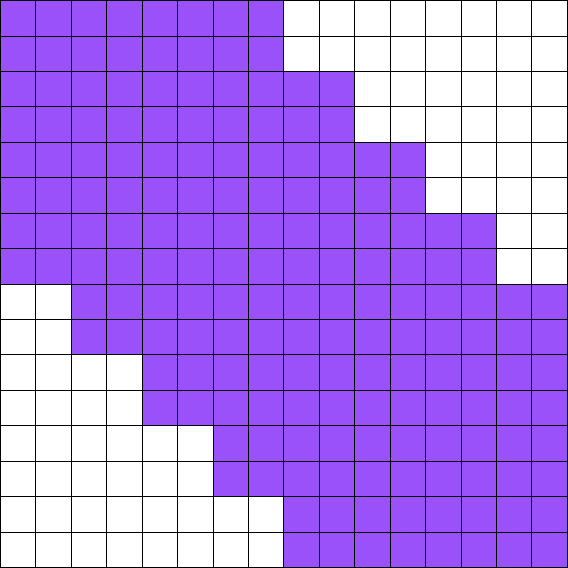
\includegraphics[width=\linewidth]{NS-LB_extraction}
        \caption{Non-symmetric B\'ezier $\bar{B}$}
        %\label{}
    \end{subfigure}
    \caption{Illustrations of the structure of $2^{nd}$ order Timoshenko beam stiffness matrices for (a) a standard displacement method, (b) a global $\bar{B}$ method, (c) a symmetric B\'ezier $\bar{B}$ method and (d) a non-symmetric B\'ezier $\bar{B}$ method.}
    \label{fig:stiffness_matrix}
\end{figure}

The increased bandwidth of the {symmetric} B\'ezier $\bar{B}$ method when compared to a displacement-based method can be explained by looking at the product of the integrals in \eqref{eqn:shear_stiffness}. For example, if we consider the basis functions $N_{1}$ and $N_{5}$ in Figure~\ref{fig:IGAelement} we see that $\operatorname{supp}(N_{1}) \cap{} \operatorname{supp}(N_{5}) = \emptyset$, which means that the inner product of these two functions will be zero and the corresponding coefficient in the stiffness matrix will be zero in the displacement-based method. For the B\'ezier $\bar{B}$ method, however, the form of \eqref{eqn:shear_stiffness} leads to a coupling between $N_{1}$ and $N_{5}$. This can be seen by considering $\Omega_2$. Over this element, the shear stiffness can be represented as
\begin{align}
	\bar{\mathbf{K}}^s_2 = \sum_{i=1}^3 \sum_{j=1}^3 \mathbf{P}_i^T\bar{\mathbf{M}}_2\mathbf{P}_j
\end{align}
and the term of this summation that results in the coupling between $N_{1}$ and $N_{5}$ is $\mathbf{P}_1^T\bar{\mathbf{M}}_2\mathbf{P}_3$, where $\mathbf{P}_1$ is the inner product of $N_{1}$ and $\hat{\bar{N}}_{2}$, $\mathbf{P}_3$ is the inner product of $N_{5}$ and $\hat{\bar{N}}_{3}$, and $\bar{\mathbf{M}}_2$ is the inner product of $\bar{N}_{2}$ and $\bar{N}_{3}$. We can see from Figure~\ref{fig:IGAelement} that $\operatorname{supp}(N_{1})\cap{}\operatorname{supp}(\hat{\bar{N}}_{2})=\Omega_1$, $\operatorname{supp}(N_{5})\cap{}\operatorname{supp}(\hat{\bar{N}}_{3})=\Omega_3$ and $\operatorname{supp}(\bar{N}_{2})\cap{}\operatorname{supp}(\bar{N}_{3})=\Omega_2$, so that $\mathbf{P}_1^T\bar{\mathbf{M}}_2\mathbf{P}_3$ is not zero. Thus we have increased the number of nonzero coefficients in the shear stiffness matrix. However, the same exercise can be used to show that there is no coupling between $N_{0}$ and $N_{6}$ for this set of basis functions so the matrix is not dense. {the bandwidth of the non-symmetric B\'ezier $\bar{B}$ method is reduced further. This is because the Gramian matrix does not appear in the this formulation.} In fact, from the formulation of the element stiffness matrix, we can show that the bandwidth of the stiffness matrix of the symmetric B\'ezier $\bar{B}$ and non-symmetric B\'ezier $\bar{B}$ methods for the Timoshenko beam are $6p-3$ and $4p-1$, respectively. 

\paragraph{Remark} In \cite{bouclier_efficient_2013} a local $\bar{B}$ method for shells was proposed that was based on the local least squares method presented in \cite{govindjee_convergence_2012}. This approach has a similar structure to the {symmetric B\'ezier $\bar{B}$} method presented here. However, it was shown in~\cite{thomas_bezier_2015} that choosing (\ref{eq:Bezier_weight}) as the weighting provides a significant increase in the accuracy of the approximation.

\begin{figure}[htb!]
      \centering
      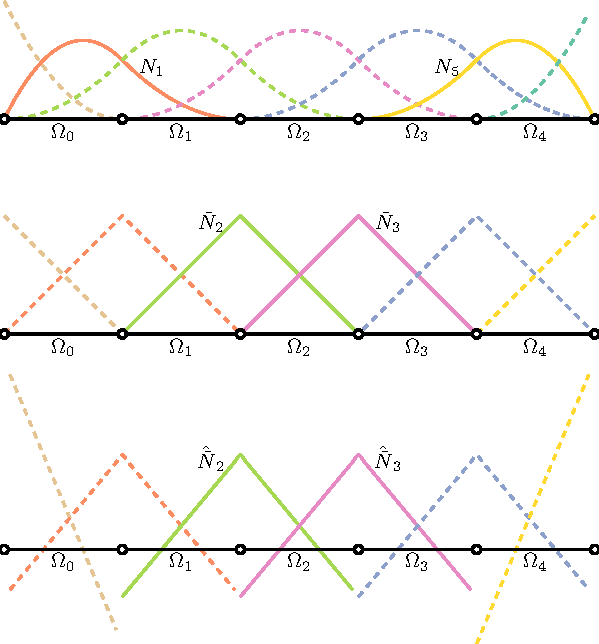
\includegraphics[width=.7\linewidth]{basis_dual}
\caption{Quadratic maximally smooth B-spline basis functions (top), associated linear basis functions (middle), and dual basis functions (bottom) for the B\'ezier $\bar{B}$ formulation.}
\label{fig:IGAelement}
\end{figure}

\subsection{Numerical results}

In our study, a straight planar cantilever beam is clamped on the left end and a sinusoidal distributed load $f(x)=sin(\pi\dfrac{x}{l})$ is applied, as depicted in Figure \ref{fig:load_beam}. The analytical solution for vertical displacement $w$, rotation $\phi$, bending moment $M$, and transverse shear force $Q$ are given by
\begin{align}
\begin{split}
w(x)&=\frac{EI\left(6 \pi ^2 l^2 \sin \left(\frac{\pi  x}{l}\right)+6 \pi ^3 l x\right)+sGA\left(6 l^4 \sin \left(\frac{\pi  x}{l}\right)-6 \pi l^3 x+3 \pi ^3 l^2 x^2-\pi ^3 l x^3\right)}{6 \pi ^4 sEIGA}\\
\phi(x)&=\frac{2 l^3 \cos \left(\frac{\pi  x}{l}\right)-2 l^3+2 \pi ^2 l^2 x-\pi ^2 l x^2}{2 \pi ^3 EI}\\
M(x)&=\frac{l^2 \sin \left(\frac{\pi  x}{l}\right)-\pi  l^2+\pi  l x}{\pi ^2}\\
Q(x)&=\frac{-l\cos \left(\frac{\pi  x}{l}\right)-l}{\pi}.
\end{split}
\label{eq:timoshenko_analytical}
\end{align}
\begin{figure}[h]
	\centering
	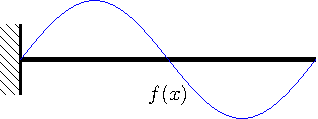
\includegraphics[width=0.4\linewidth]{beam_load}
	\caption{Straight planar cantilevered Timoshenko beam clamped at the left and loaded by a distributed load $f(x)$.}
	\label{fig:load_beam}
\end{figure}

The beam has a rectangular cross-section and we use the following non-dimensional sectional and material parameters: length $l=10$, width $b=1$, thickness $t=0.01$, Young's modulus $E=10^9$, Poisson's ratio $\nu=0.3$, and a shear correction factor of $s=5/6$. A comparison of the normalized error in the $L^2$ norm for $w$, $\phi$, $M$ and $Q$ versus the number of degrees of freedom for polynomial degrees $p=1,2,3$ is shown in Figure \ref{fig:timoshenko_result}. Results computed using standard finite elements are labeled $Q_1$, $Q_2$, and $Q_3$. Results computed using a global $\bar{B}$ method are labeled $\mathcal{T}^{L^2}$, those computed with the symmetric B\'ezier $\bar{B}$ method and the non-symmetric B\'ezier $\bar{B}$ method are labeled $S-\mathcal{T}^{P}$ and $NS-\mathcal{T}^{P}$, respectively. As expected, the $Q_1$ results lock and the error remains virtually unchanged as the mesh is refined. Increasing the polynomial degree does reduce the locking effect, although the reduction is minor for the $Q_2$ results. $\mathcal{T}^{L^2}$, $S-\mathcal{T}^{P}$ and $NS-\mathcal{T}^P$ are essentially locking free for all polynomial orders. The convergence rates for the $\bar{B}$ methods are at least $p+1$ for $w$, $p$ for $\phi$, $p-1$ for $M$, and $p-2$ for $Q$. These rates agree with those reported in \cite{kiendl_single-variable_2015} and are optimal. To reiterate, B\'{e}zier $\bar{B}$ methods produces the same convergence rates as the global $\bar{B}$ method {and the the error plots of $NS-\mathcal{T}^{P}$ for $\phi$, $M$ and $Q$ are identical to those of $\mathcal{T}^{L^2}$}.
\begin{figure}
    \centering
    \begin{subfigure}[b]{0.49\linewidth}        %% or \columnwidth
        \centering
        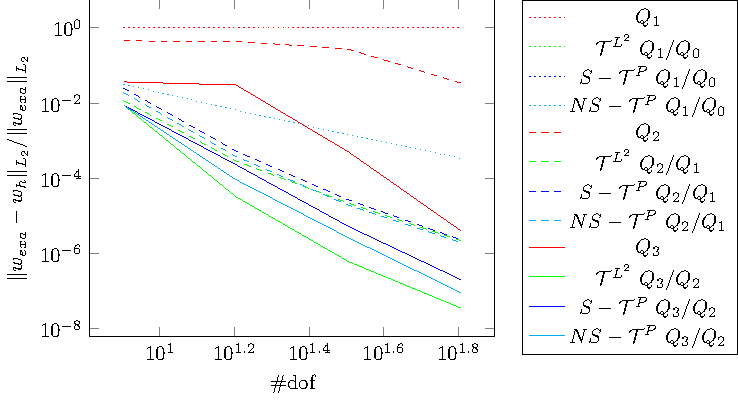
\includegraphics[width=\linewidth]{w-sin}
        \caption{}
        \vspace*{2mm}
    \end{subfigure}
    \begin{subfigure}[b]{0.49\linewidth}        %% or \columnwidth
        \centering
        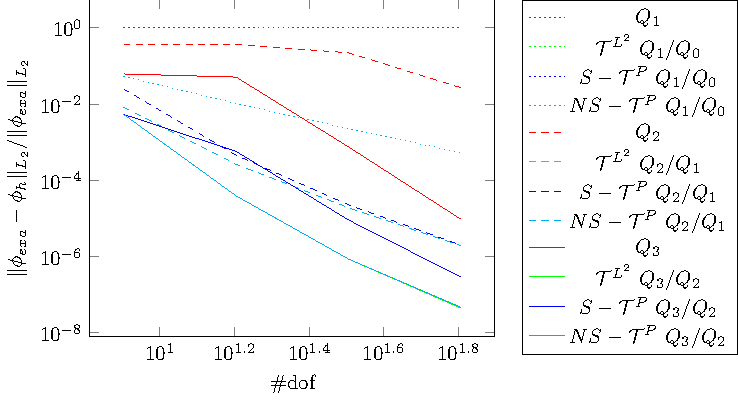
\includegraphics[width=\linewidth]{phi-sin}
        \caption{}
        \vspace*{2mm}
    \end{subfigure}
        \begin{subfigure}[b]{0.49\linewidth}        %% or \columnwidth
        \centering
        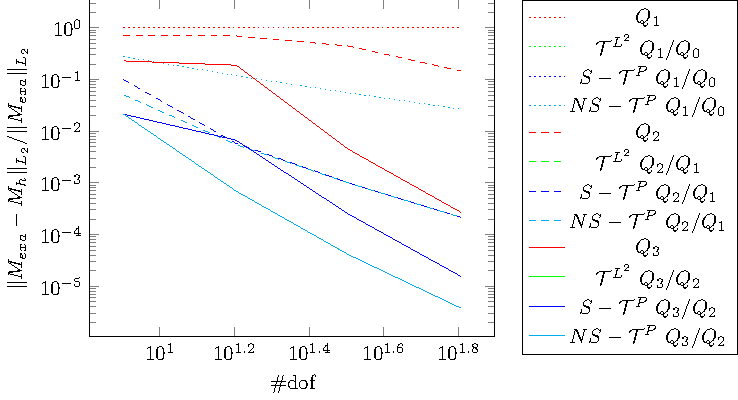
\includegraphics[width=\linewidth]{M-sin}
        \caption{}
        \vspace*{2mm}
    \end{subfigure}
    \begin{subfigure}[b]{0.49\linewidth}        %% or \columnwidth
        \centering
        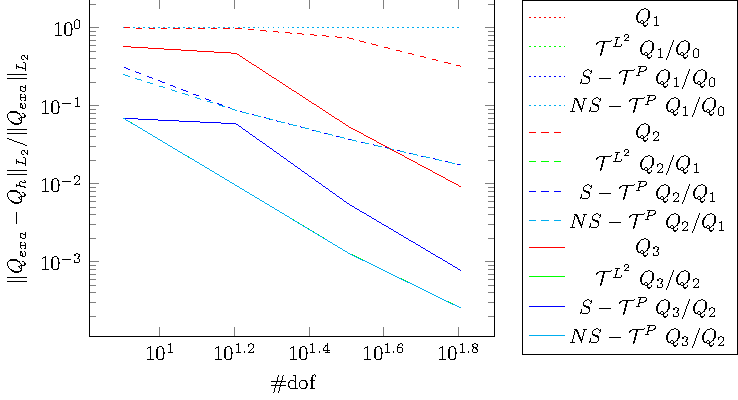
\includegraphics[width=\linewidth]{Q-sin}
        \caption{}
        \vspace*{2mm}
    \end{subfigure}
    \caption{Convergence studies for slenderness factor $l/t=10^{-3}$. Error in the $L^2$-norm for (a) displacement $w$, (b) rotation $\phi$, (c) bending moment $M$, and (d) shear force $Q$.}
    \label{fig:timoshenko_result}
\end{figure}

We have also studied the relationship between shear locking and decreasing slenderness ratios for $p=2$. The results are shown in Figure \ref{fig:slenderness}. For all three methods, the number of degrees of freedom are fixed, and the sectional and material parameters are the same as in the previous study. The slenderness ratio varies from $10$ to $5\times{10}^3$. $Q_2$ locks severely. The $\bar{B}$ methods, on the other hand, are locking free. 
%Note that the jump in the error for at the largest slenderness for the $\bar{B}$ methods is due to numerical round-off errors. If the computation is performed with high precision floating point numbers this jump is not present.

\begin{figure}
    \centering
    \begin{subfigure}[b]{0.49\linewidth}        %% or \columnwidth
        \centering
        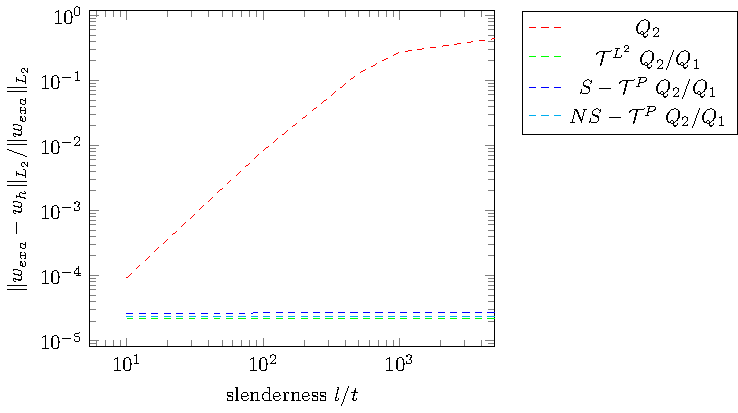
\includegraphics[width=\linewidth]{slenderness_w}
        \caption{}
        \vspace*{2mm}
    \end{subfigure}
    \begin{subfigure}[b]{0.49\linewidth}        %% or \columnwidth
        \centering
        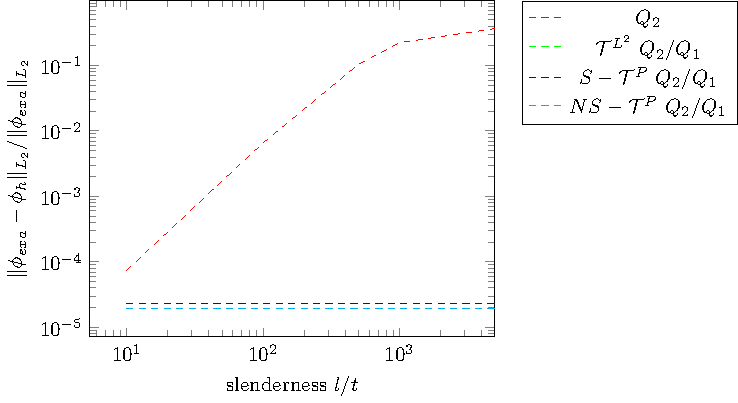
\includegraphics[width=\linewidth]{slenderness_phi}
        \caption{}
        \vspace*{2mm}
    \end{subfigure}
        \begin{subfigure}[b]{0.49\linewidth}        %% or \columnwidth
        \centering
        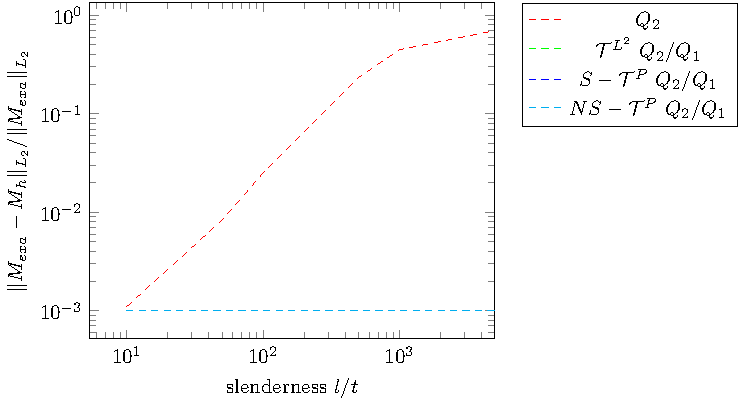
\includegraphics[width=\linewidth]{slenderness_M}
        \caption{}
        \vspace*{2mm}
    \end{subfigure}
    \begin{subfigure}[b]{0.49\linewidth}        %% or \columnwidth
        \centering
        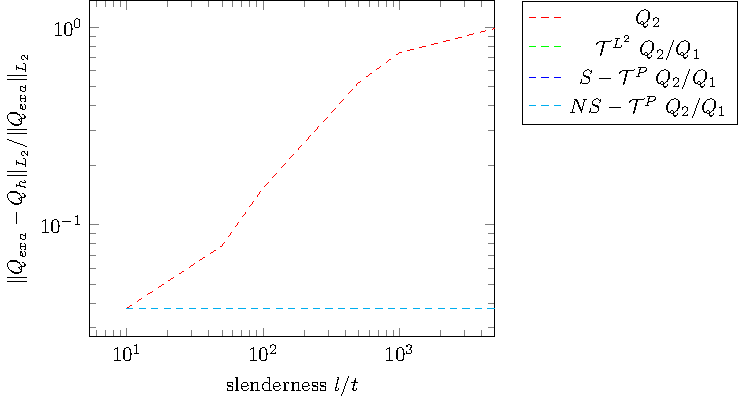
\includegraphics[width=\linewidth]{slenderness_Q}
        \caption{}
        \vspace*{2mm}
    \end{subfigure}
    \caption{Convergence study for increasing slenderness, $p=2$, and $\#{dof}=32$. Error in the $L^2$-norm for (a) displacement $w$, (b) rotation $\phi$, (c) bending moment $M$, and (d) shear force $Q$.}
    \label{fig:slenderness}
\end{figure}


\section{Volumetric locking: Nearly incompressible linear elasticity}
\label{sec:nearlyincompressible}
To demonstrate the use of \Bezier $\bar{B}$ {methods} to alleviate volumetric locking effects we study the nearly incompressible elasticity problem in two dimensions. We start with the small strain tensor $\boldsymbol{\varepsilon}$, which is defined as the symmetric part of the displacement gradient, i.e., 
\begin{equation}
\varepsilon_{ij}=\dfrac{u_{i,j}+u_{j,i}}{2}.
\end{equation}
The stress tensor is related to the strain tensor through the generalized Hooke's law
\begin{equation}
\sigma_{ij}=c_{ijkl}\varepsilon_{kl}
\end{equation}
where, for isotropic elasticity, the elastic coefficients and stress tensor can be expressed in terms of the Lam\'{e} parameters $\lambda$ and $\mu$ as
\begin{align}
c_{ijkl} &=\mu(\delta_{ik}\delta_{jl}+\delta_{il}\delta_{jk})+\lambda\delta_{ij}\delta_{kl}\\
\sigma_{ij} &= \lambda\varepsilon_{kk}\delta_{ij} + 2\mu\varepsilon_{ij}.
\end{align}
The Lam\'e parameters $\lambda$ and $\mu$ are defined in terms of Young's modulus, $E$, and Poisson's ratio, $\nu$, as
\begin{align}
\lambda &=\dfrac{\nu{E}}{(1+\nu)(1-2\nu)}\\
\mu &=\dfrac{\nu{E}}{2(1+\nu)}.
\end{align}
we can write the strong form of linear elasticity as
\begin{align}
	\sigma_{ij,j}+f_i &= 0 \text{ in $\Omega$} \\
    u_i &= g_i\text{ on $\Gamma_{g_i}$} \\
    \sigma_{ij}n_j &= h_i\text{ on $\Gamma_{h_i}$}
\end{align}
where Dirichlet boundary conditions are applied on $\Gamma_{g_i}$, Neumann boundary conditions are applied on $\Gamma_{h_i}$, and the closure of the domain $\Omega$ is $\bar{\Omega}=\Omega\cup\Gamma_{g_i}\cup\Gamma_{h_i}$. {To demonstrate the source of volumetric locking, we introduce the pressure term}
\begin{equation}
    p=-(\lambda+2\mu/3){\epsilon}_{ii}.
\end{equation}
If $\nu\rightarrow\dfrac{1}{2}$ then $\lambda$ becomes very large and {the additional constraint $\epsilon_{ii} = 0$ is applied to the volumetric strain.}

\subsection{Symmetric \Bezier $\bar{B}$ projection}
\subsubsection{The weak form}
The $\bar{B}$ approach for nearly incompressible linear elasticity splits the strain tensor $\varepsilon$ into volumetric and deviatoric strains and then replaces the volumetric strain with a projected strain. We begin with
\begin{equation}
\boldsymbol{\varepsilon}(\mathbf{u})=\boldsymbol{\varepsilon}^{vol}(\mathbf{u})+\boldsymbol{\varepsilon}^{dev}(\mathbf{u})
\end{equation}
where $\boldsymbol{\varepsilon}^{vol}=\dfrac{1}{3}\mathrm{tr}(\boldsymbol{\varepsilon})\mi$ is the volumetric strain and $\boldsymbol{\varepsilon}^{dev}=\boldsymbol{\varepsilon}-\dfrac{1}{3}\mathrm{tr}(\boldsymbol{\varepsilon})\mi$ is the deviatoric strain. The volumetric strain is then replaced by a projected volumetric strain $\bar{\boldsymbol{\varepsilon}}^{vol}$ and the new total strain becomes
\begin{equation}
\bar{\boldsymbol{\varepsilon}}=\bar{\boldsymbol{\varepsilon}}^{vol}+\boldsymbol{\varepsilon}^{dev}.
\end{equation}
The weak form can then be written as: find $\mathbf{u}\in{\mathcal{S}(\Omega)}$ such that for all $\mathbf{w}\in{\mathcal{V}(\Omega)}$
\begin{equation}
    \bar{a}\langle{\mathbf{w},\mathbf{u}}\rangle=\bar{l}\langle{\mathbf{w}}\rangle
\end{equation}
where
\begin{align}
    \bar{a}\langle{\mathbf{w},\mathbf{u}}\rangle&=\int_{\Omega}\bar{\epsilon}_{ij}(\mathbf{w})c_{ijkl}\bar{\epsilon}_{kl}(\mathbf{u})d\Omega, \\
    \bar{l}\langle{\mathbf{w}}\rangle&=\int_{\Omega}\mathbf{w}\cdot\mathbf{f}d\Omega+\int_{\Gamma_{h}}\mathbf{w}\cdot\mathbf{h}d\Gamma.
\end{align}

\subsubsection{Discretization}
Following the same approach as was described for Timoshenko beams in Section~\ref{sec:timoshenkobeam} we define element level strain-displacement matrices in terms of the Bernstein basis 
\begin{align}
{\mathbf{B}^{dev}_e}&=
\begin{bmatrix}
\dfrac{2}{3}\dfrac{\partial{B}^e_{0,p}}{\partial{x}} & -\dfrac{1}{3}\dfrac{\partial{B}^e_{0,p}}{\partial{y}} & -\dfrac{1}{3}\dfrac{\partial{B}^e_{0,p}}{\partial{z}} & \cdots & \dfrac{2}{3}\dfrac{\partial{B}^e_{p,p}}{\partial{x}} & -\dfrac{1}{3}\dfrac{\partial{B}^e_{p,p}}{\partial{y}} & -\dfrac{1}{3}\dfrac{\partial{B}^e_{p,p}}{\partial{z}} \\
-\dfrac{1}{3}\dfrac{\partial{B}^e_{0,p}}{\partial{x}}  & \dfrac{2}{3}\dfrac{\partial{B}^e_{0,p}}{\partial{y}} & -\dfrac{1}{3}\dfrac{\partial{B}^e_{0,p}}{\partial{z}} & \cdots & -\dfrac{1}{3}\dfrac{\partial{B}^e_{p,p}}{\partial{x}}  & \dfrac{2}{3}\dfrac{\partial{B}^e_{p,p}}{\partial{y}} & -\dfrac{1}{3}\dfrac{\partial{B}^e_{p,p}}{\partial{z}}\\
-\dfrac{1}{3}\dfrac{\partial{B}^e_{0,p}}{\partial{x}} & -\dfrac{1}{3}\dfrac{\partial{B}^e_{0,p}}{\partial{y}} & \dfrac{2}{3}\dfrac{\partial{B}^e_{0,p}}{\partial{z}} & \cdots & -\dfrac{1}{3}\dfrac{\partial{B}^e_{p,p}}{\partial{x}} & -\dfrac{1}{3}\dfrac{\partial{B}^e_{p,p}}{\partial{y}} & \dfrac{2}{3}\dfrac{\partial{B}^e_{p,p}}{\partial{z}}\\
0 & \dfrac{\partial{B}^e_{0,p}}{\partial{z}} & \dfrac{\partial{B}^e_{0,p}}{\partial{y}} & \cdots & 0 & \dfrac{\partial{B}^e_{p,p}}{\partial{z}} & \dfrac{\partial{B}^e_{p,p}}{\partial{y}}\\
\dfrac{\partial{B}^e_{0,p}}{\partial{z}} & 0 & \dfrac{\partial{B}^e_{0,p}}{\partial{x}} & \cdots & \dfrac{\partial{B}^e_{p,p}}{\partial{z}} & 0 & \dfrac{\partial{B}^e_{p,p}}{\partial{x}}\\
\dfrac{\partial{B}^e_{0,p}}{\partial{y}} & \dfrac{\partial{B}^e_{0,p}}{\partial{x}} & 0 & \cdots & \dfrac{\partial{B}^e_{p,p}}{\partial{y}} & \dfrac{\partial{B}^e_{p,p}}{\partial{x}} & 0\\
\end{bmatrix},
\end{align}
\begin{align}
{\mathbf{B}_e^{vol}}&=
\begin{bmatrix}
\dfrac{\partial{B}^e_{0,p}}{\partial{x}} & \dfrac{\partial{B}^e_{0,p}}{\partial{y}} & \dfrac{\partial{B}^e_{0,p}}{\partial{z}} & \cdots & \dfrac{\partial{B}^e_{p,p}}{\partial{x}} & \dfrac{\partial{B}^e_{p,p}}{\partial{y}} & \dfrac{\partial{B}^e_{p,p}}{\partial{z}}
\end{bmatrix}
\end{align}
The deviatoric part of the element stiffness matrix can then be computed from the corresponding strain-displacement matrices as
\begin{align}
	\mathbf{K}_e^{dev}
    	=\mathbf{C}^e\langle {\mathbf{B}_{e}^{dev}}^T\mathbf{D}{\mathbf{B}}_{e}^{dev}\rangle (\mathbf{C}^e)^T.
\end{align}
where $\mathbf{C}^e$ is the element extraction operator for the degree $p$ spline space. The volumetric part of the stiffness matrix is computed using Bezier projection. The intermediate element matrices are
\begin{align}
\bar{\mathbf{M}}^{vol}_e&=\bar{\mathbf{C}}^e\langle{\bar{\mathbf{B}}_e^T,\dfrac{1}{3}(3\lambda+2\mu)\bar{\mathbf{B}}_e}\rangle(\bar{\mathbf{C}}^e)^T\\
\hat{\mathbf{P}}^{vol}_e&=\langle{(\hat{\bar{\mathbf{N}}}^e)^T, \mathbf{B}_e^{vol}}\rangle(\mathbf{C}^e)^T
\end{align}
where $\bar{\mathbf{C}}^e$ is the element extraction operator for the degree $p-1$ spline space, $\hat{\bar{\mathbf{N}}}^e$ are the dual basis functions restriced to the element, and \begin{equation}
\bar{\mathbf{B}}_e=
\begin{bmatrix}
{B}^e_{0,p-1} & \cdots & {B}^e_{p-1,p-1}
\end{bmatrix}.
\end{equation}The global stiffness matrix can then be assembled as
\begin{align}
	\mathbf{K} = \mathbf{K}^{dev} + \bar{\mathbf{K}}^{vol}_{S}
\end{align}
where
\begin{align}
	\mathbf{K}^{dev} &=\A_e\mathbf{K}_e^{dev}, \\
	\bar{\mathbf{K}}_S^{vol}&=\hat{\mathbf{P}}^T\bar{\mathbf{M}}\hat{\mathbf{P}} \\
	\hat{\mathbf{P}} &=\A_e\hat{{\mathbf{P}}}^{vol}_e \\
    \bar{\mathbf{M}} &=\A_e\bar{\mathbf{M}}^{vol}_e.
\end{align}
\subsection{Non-symmetric \Bezier $\bar{B}$ projection}
\subsubsection{The weak form}
{A mixed formulation for nearly incompressible elasticity can be developed by considering the pressure $p$ as an independent variable. The weak statement of the problem is then given as: find $\mathbf{u}\in{\mathcal{S}(\Omega)}$ and $p\in{L}^2(\Omega)$ such that for all $\mathbf{w}\in{\mathcal{V}(\Omega)}$ and $\delta{p}\in{L}^2(\Omega)$}
\begin{align}
    \hat{a}\langle{\mathbf{w},\mathbf{u}}\rangle-b\langle{\mathbf{w},p}\rangle&=l\langle{\mathbf{w}}\rangle, \\
    - b\langle{\mathbf{u},\delta{p}}\rangle-\dfrac{1}{(\lambda+2\mu/3)}\int_{\Omega}\delta{p}pd\Omega&=0,
\end{align}
where
\begin{align}
    \hat{a}\langle{\mathbf{w},\mathbf{u}}\rangle&=\int_{\Omega}\epsilon_{ij}(\mathbf{w})\hat{c}_{ijkl}\epsilon_{kl}(\mathbf{u})d\Omega,\\
    \hat{c}_{ijkl}&=\mu\left(\delta_{ik}\delta_{jl}+\delta_{il}\delta_{jk}-2/3\delta_{ij}\delta_{kl}\right),\\
    b\langle{\mathbf{w},p}\rangle&=\int_{\Omega}\epsilon_{ii}(\mathbf{w})pd\Omega.
\end{align}

\subsubsection{{Discretization}}

Following the same pattern as the non-symmetric \Bezier $\bar{B}$ method for the Timoshenko beam problem, we use the same discretization for $\mathbf{u}$ and $\mathbf{w}$ and use lower order spline basis functions and corresponding dual basis functions for the discretization of the pressure $p$ and its variation $\delta{p}$, respectively. The discretized stiffness matrix in mixed form can be written as
\begin{equation}
    \mathbf{K}_{mix}=
    \begin{bmatrix}
        \mathbf{K}^{dev} & -\mathbf{P}^{T}\\
        -\hat{\mathbf{P}} & -\dfrac{1}{(\lambda+2\mu/3)}\mathbf{I}
    \end{bmatrix},
\end{equation}
{where}
\begin{equation}
    \mathbf{P}=\A_e\mathbf{P}_e^{vol},
\end{equation}
with
\begin{equation}
    \mathbf{P}_e^{vol}=\bar{\mathbf{C}}^e\langle{\bar{\mathbf{B}}_e^T,\mathbf{B}^{vol}_e}\rangle(\mathbf{C}^e)^T.
\end{equation}
By eliminating the pressure control variables, we obtain a pure displacement formulation with the stiffness matrix taking the form
\begin{equation}
	\mathbf{K} = \mathbf{K}^{dev} + \bar{\mathbf{K}}^{vol}_{NS},
\end{equation}
where
\begin{equation}
    \bar{\mathbf{K}}^{vol}_{NS}=(\lambda+2\mu/3){\mathbf{P}}^T\hat{\mathbf{P}}.
\end{equation}
We note again, that in contrast to the symmetric \Bezier $\bar{B}$ method, the assembly of the stiffness matrix in this case can be performed in the standard way with no need for global matrix operations.
 
\subsection{Numerical results}
{We begin this section by numerically evaluating the inf��-sup constant for the global $\bar{B}$ and non-symmetric \Bezier $\bar{B}$ methods.} 
We then investigate the performance of the B\'{e}zier $\bar{B}$ method for two nearly incompressible linear elasticity problems under plane strain conditions. {For the numerical examples,} we first study the Cook's membrane problem, which is discretized with B-spline basis functions, and in the second problem we model an infinite plate with a circular hole using NURBS. Results computed using standard finite elements are labeled $Q_1$, $Q_2$, $Q_3$, and $Q_4$. Results computed using a global $\bar{B}$ method are labeled $\mathcal{T}^{L^2}$ and those computed with the {symmetric} B\'ezier $\bar{B}$ method and the {non-symmetric B\'ezier $\bar{B}$ method} are labeled $S-\mathcal{T}^{P}$ and $NS-\mathcal{T}^{P}$, respectively.

\subsubsection{{Numerical evaluation of the inf-sup condition}}

The inf-sup condition is also refered to as the Ladyzhenskaya-Babuska-Brezzi condition (or simply LBB)~\cite{babuvska1973finite, brezzi1974existence, ladyzhenskaya1969mathematical}. It is a crucial condition to ensure the solvability, stability and optimality of a mixed problem. For the nearly incompressible elasticity problem the inf-sup condition is stated as: for $\delta{p}\neq{0}$ and $\mathbf{u}\neq{0}$
\begin{equation}
    \inf_{\delta{p}\in{L^2(\Omega)}}\sup_{\mathbf{u}\in\mathcal{S}(\Omega)}\dfrac{\vert{b\langle{\mathbf{u},\delta{p}}\rangle}\vert}{\|{\delta{p}}\|_{L^2(\Omega)}\|{\mathbf{u}}\|_{H^1(\Omega)}}\geq\beta>0.
\end{equation}
In a discretized problem, the inf-sup condition requires the variable $\beta$ to be a constant that is independent of the mesh size.\par

Here, we consider the inf-sup condition of a uniformly refined quarter annulus. The geometry and boundary conditions are shown in Figure \ref{fig:quarter_annulus}. The geometry of the quarter annulus can be exactly represented using a biquadratic NURBS basis. The knot vector for the coarsest discretization is given by
\begin{align}
\begin{split}
\Xi_\xi\times\Xi_\eta=\lbrace{0,0,0,1,1,1}\rbrace\times\lbrace{0,0,0,1,1,1}\rbrace
\end{split}
\end{align}
and the corresponding weights and control points associated with each basis function are given in Table \ref{table:weights} and \ref{table:control_points}. For higher-order elements and finer discretizations the weights and corresponding control points are identified by an order elevation and knot insertion algorithm, respectively. The B\'ezier mesh representation for the discretizations are shown in Figure \ref{fig:mesh_hole}.

\begin{figure}[htb!]
	\centering
	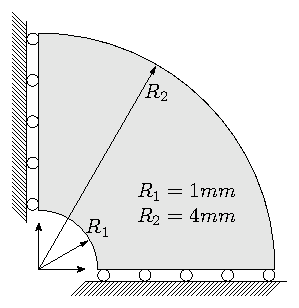
\includegraphics[width=0.5\linewidth]{annular}
	\caption{Geometry and boundary conditions for the inf-sup test.}
	\label{fig:quarter_annulus}
\end{figure}

\begin{table}
\begin{center}
\caption{Weights for the plate with a circular hole}\label{table:weights}
\begin{tabular}{l@{\hskip 1cm}l@{\hskip 1cm}l@{\hskip 1cm}l}
\hline
i    & $w_{i,1} $ & $w_{i,2}$ & $w_{i,3}$\\
\hline
1    & 1    & ${1}/{\sqrt{2}}$ & 1 \\
2    & 1    & ${1}/{\sqrt{2}}$ & 1 \\
3    & 1    & ${1}/{\sqrt{2}}$ & 1 \\
\hline
\end{tabular}
\end{center}
\end{table}

\begin{table}
\begin{center}
\caption{Control points for the plate with a circular hole}\label{table:control_points}
\begin{tabular}{l@{\hskip 1cm}l@{\hskip 1cm}l@{\hskip 1cm}l}
\hline
i    & $B_{i,1} $ & $B_{i,2}$ & $B_{i,3}$\\
\hline
1    & (0,1)    & (1,1)     & (1,0)   \\
2    & (0,2.5)  & (2.5,2.5) & (2.5,0) \\
3    & (0,4)    & (4,4)     & (4,0)   \\
\hline
\end{tabular}
\end{center}
\end{table}
\begin{figure}
    \centering
    \begin{subfigure}[b]{0.18\linewidth}        %% or \columnwidth
        \centering
        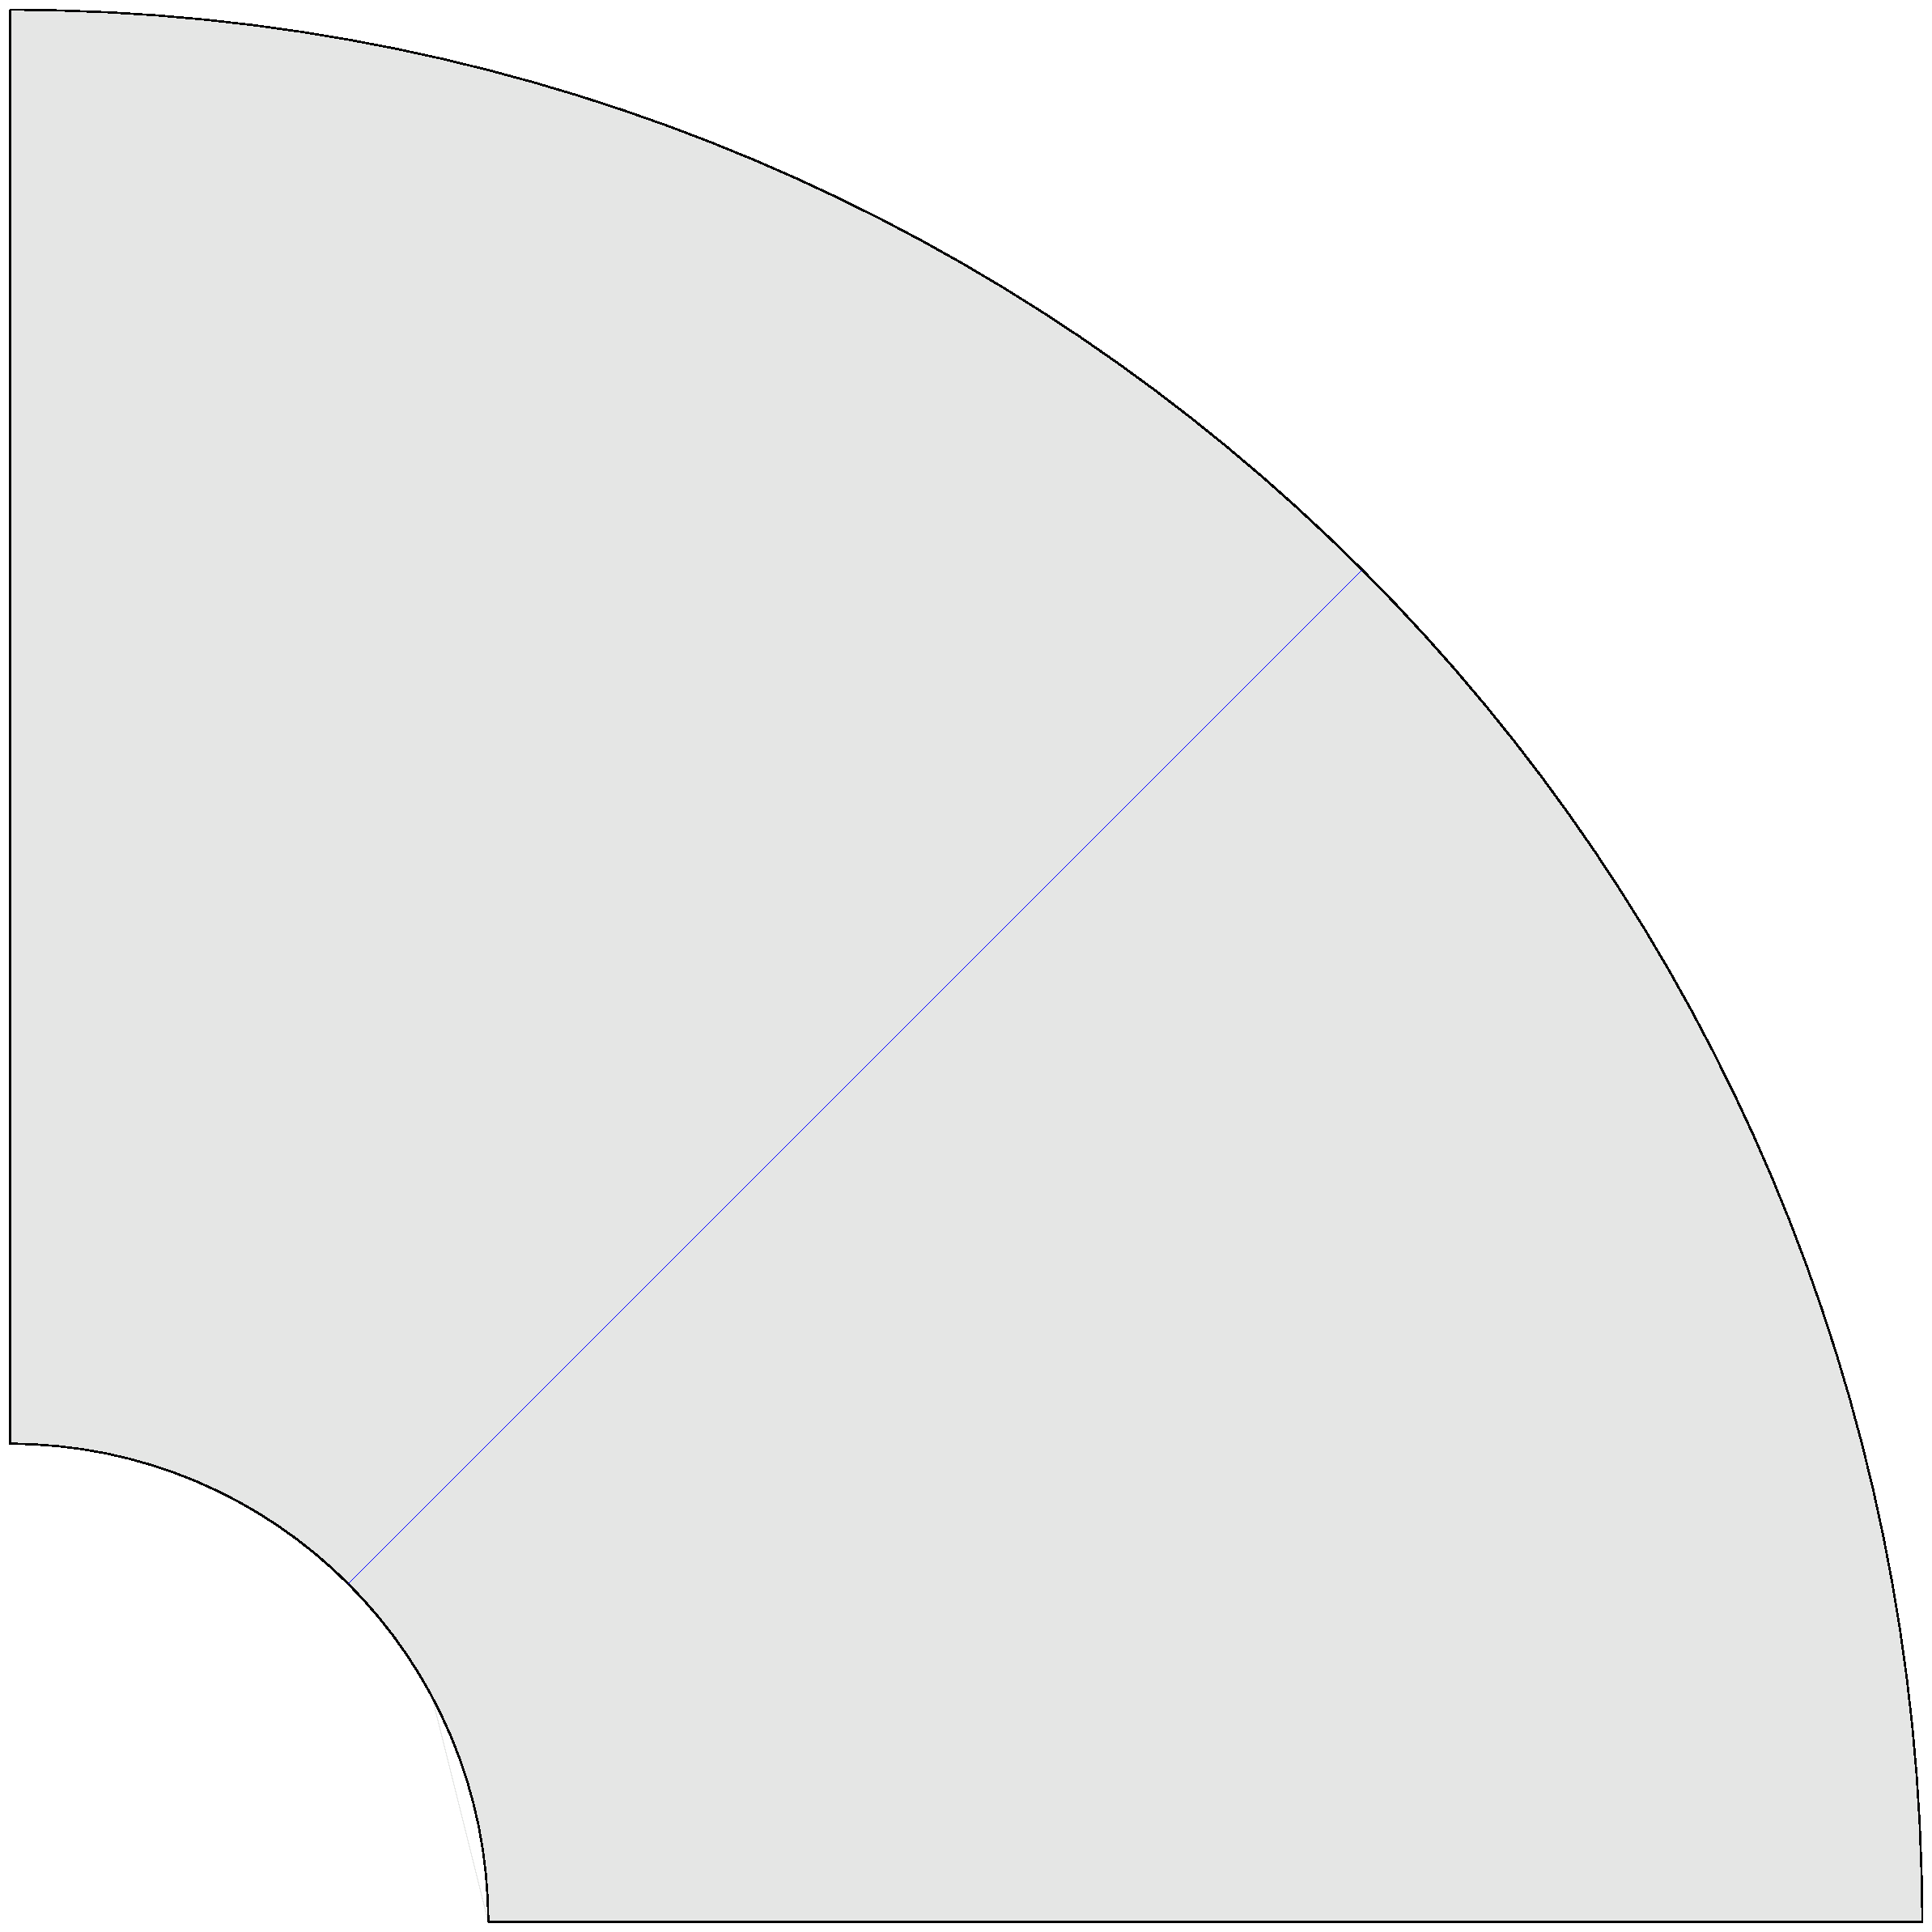
\includegraphics[width=\linewidth]{mesh_hole_0}
    \end{subfigure}
    \begin{subfigure}[b]{0.18\linewidth}        %% or \columnwidth
        \centering
        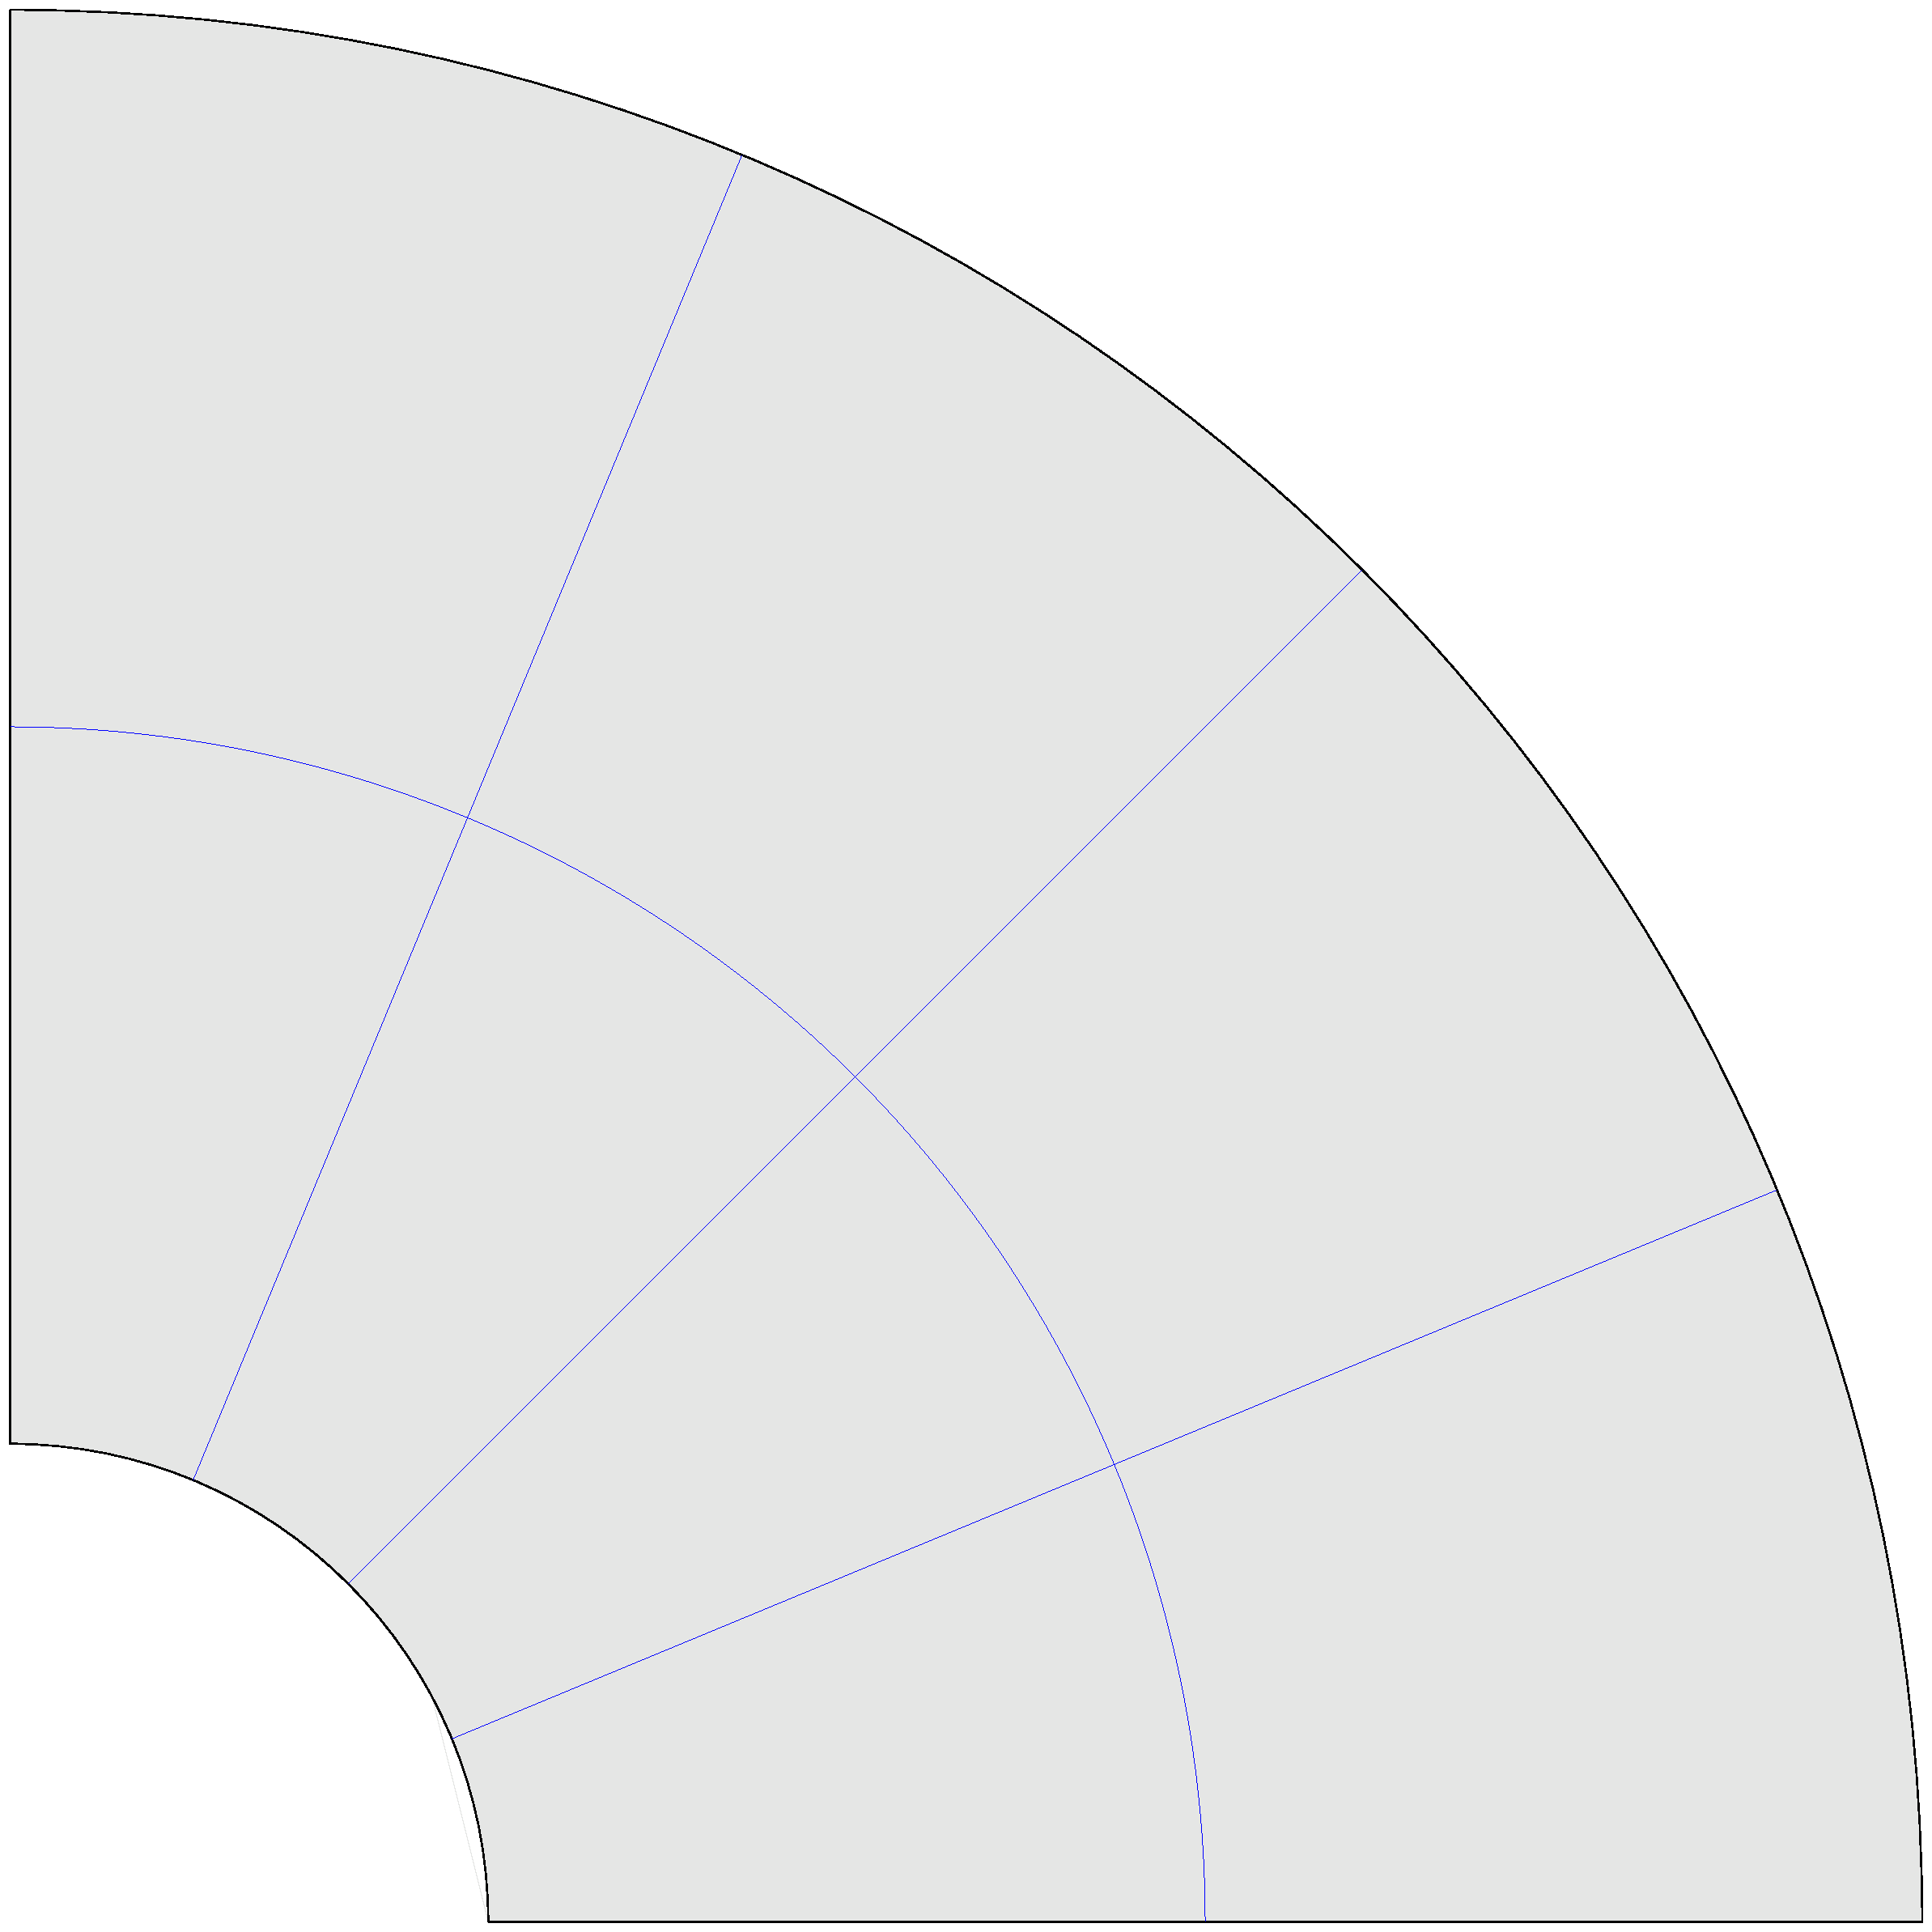
\includegraphics[width=\linewidth]{mesh_hole_1}
    \end{subfigure}
    \begin{subfigure}[b]{0.18\linewidth}        %% or \columnwidth
        \centering
        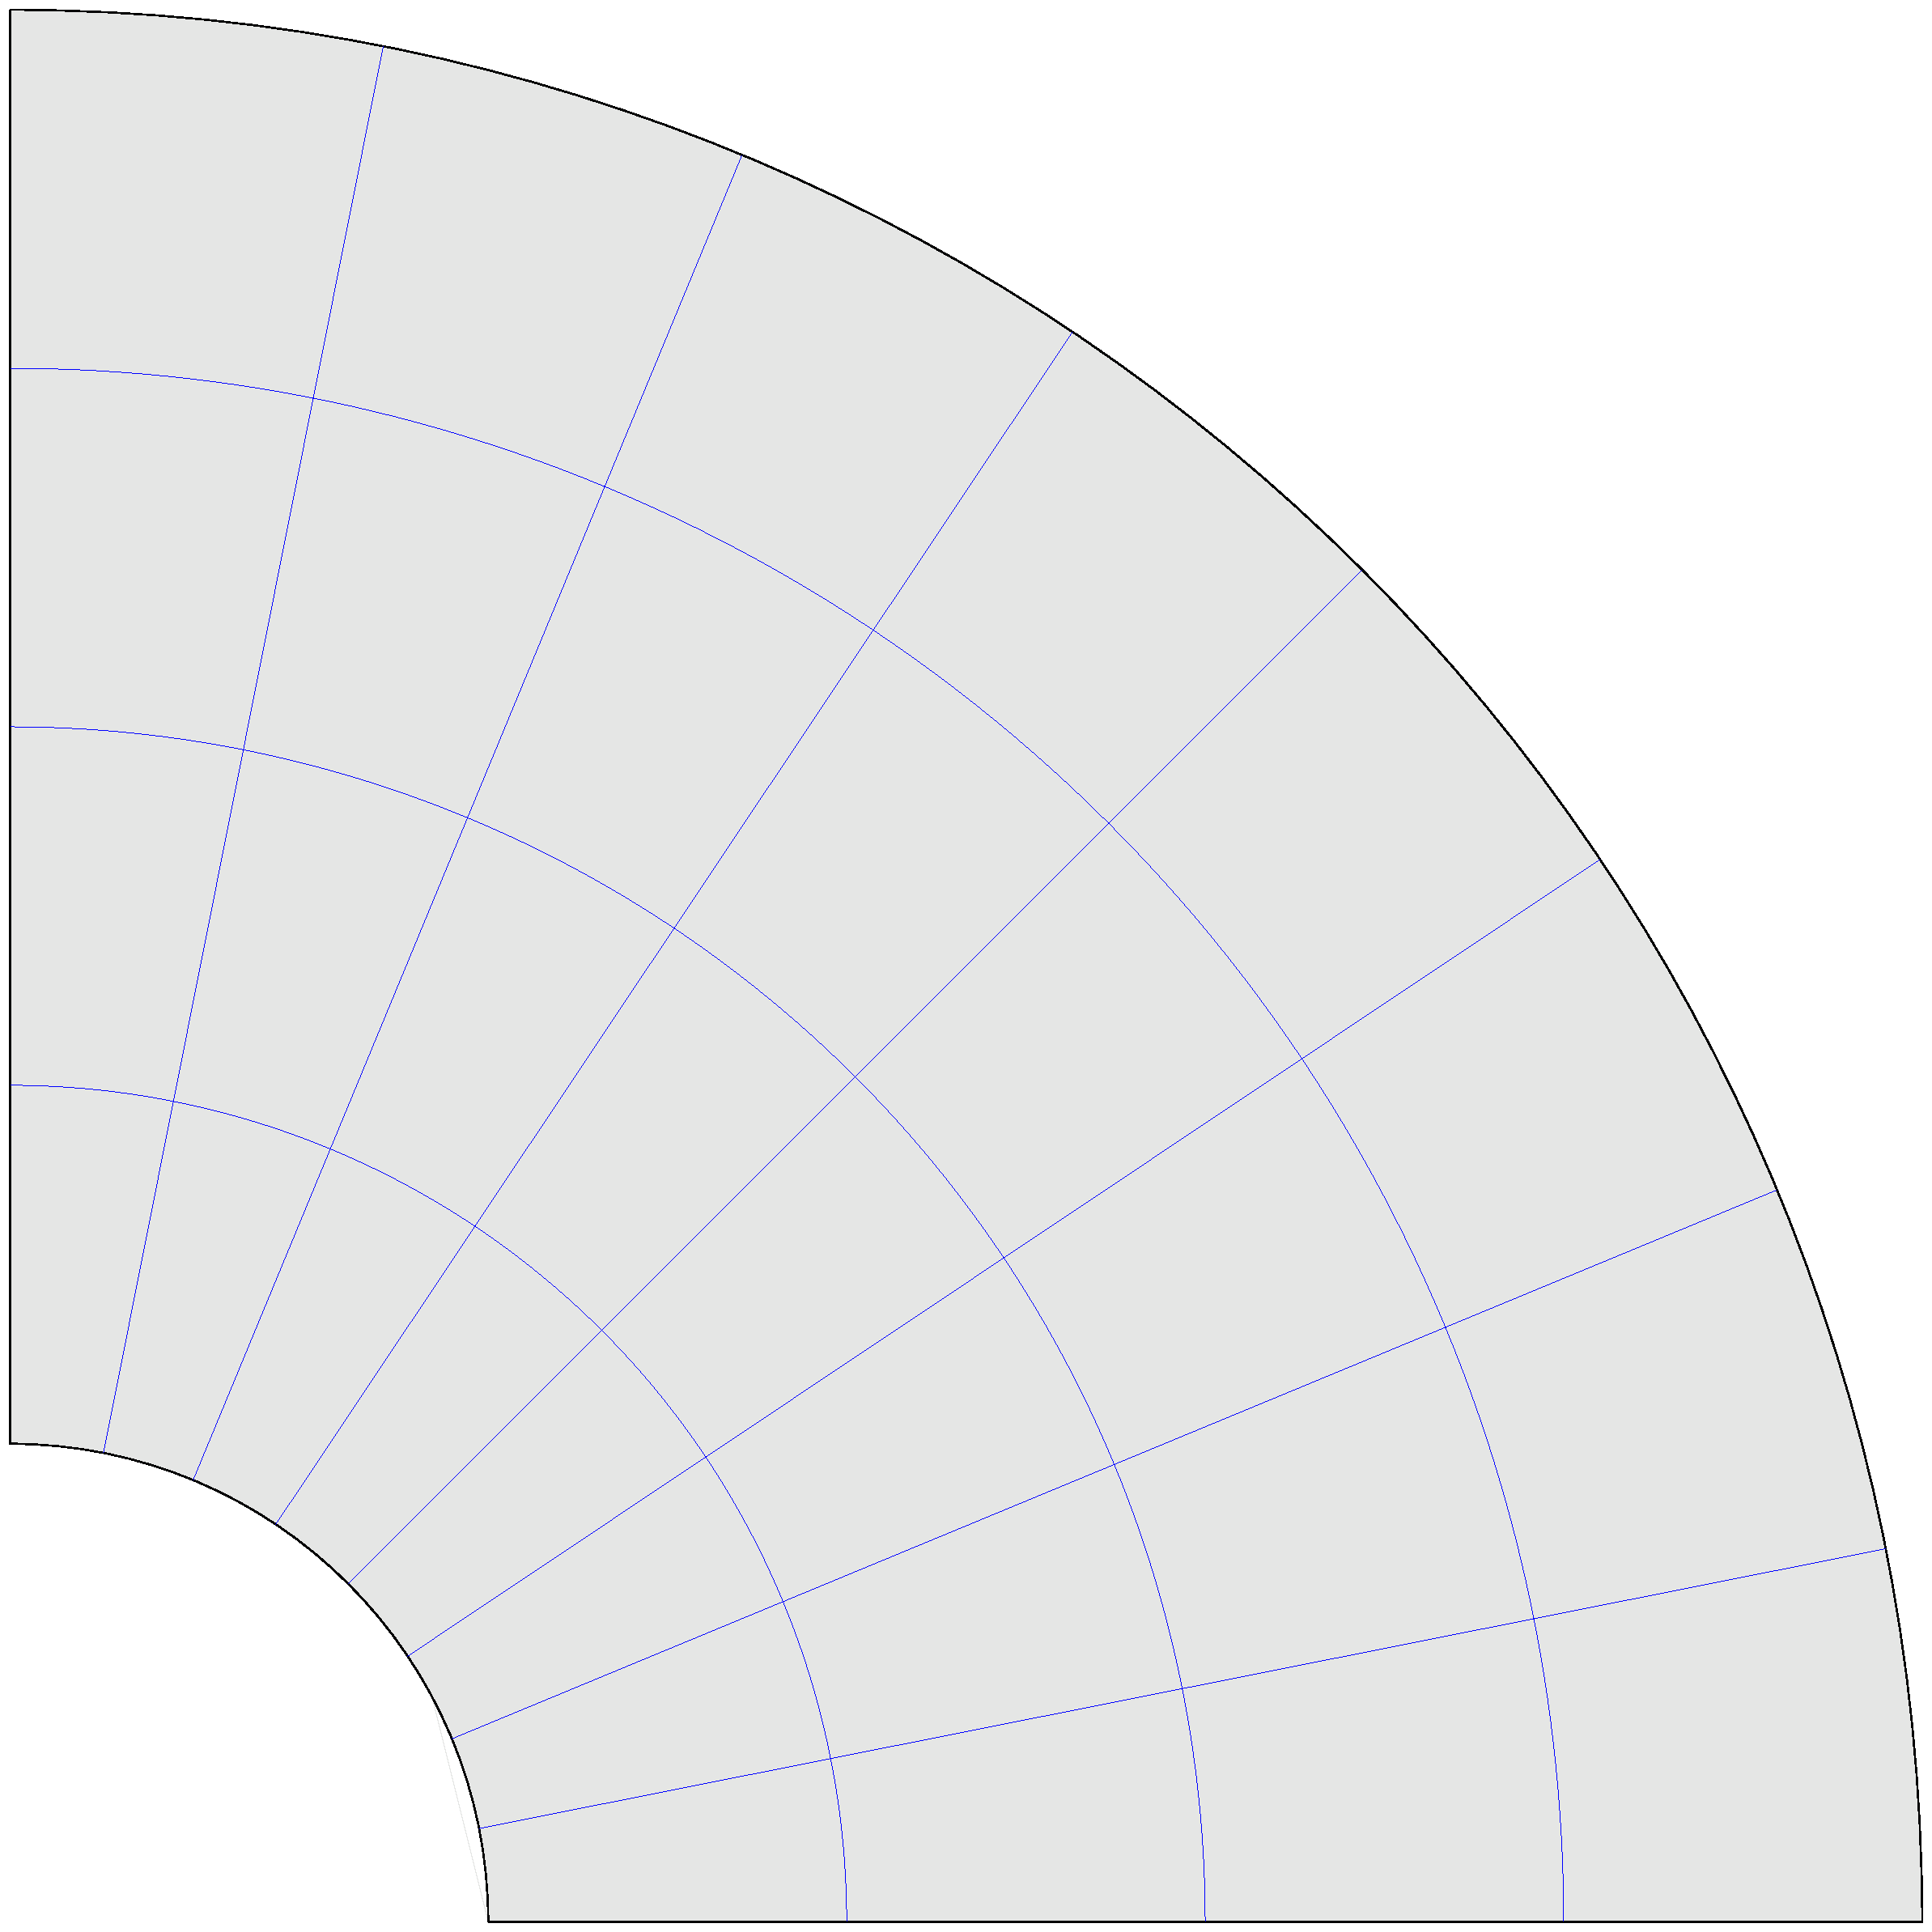
\includegraphics[width=\linewidth]{mesh_hole_2}
    \end{subfigure}
    \begin{subfigure}[b]{0.18\linewidth}        %% or \columnwidth
        \centering
        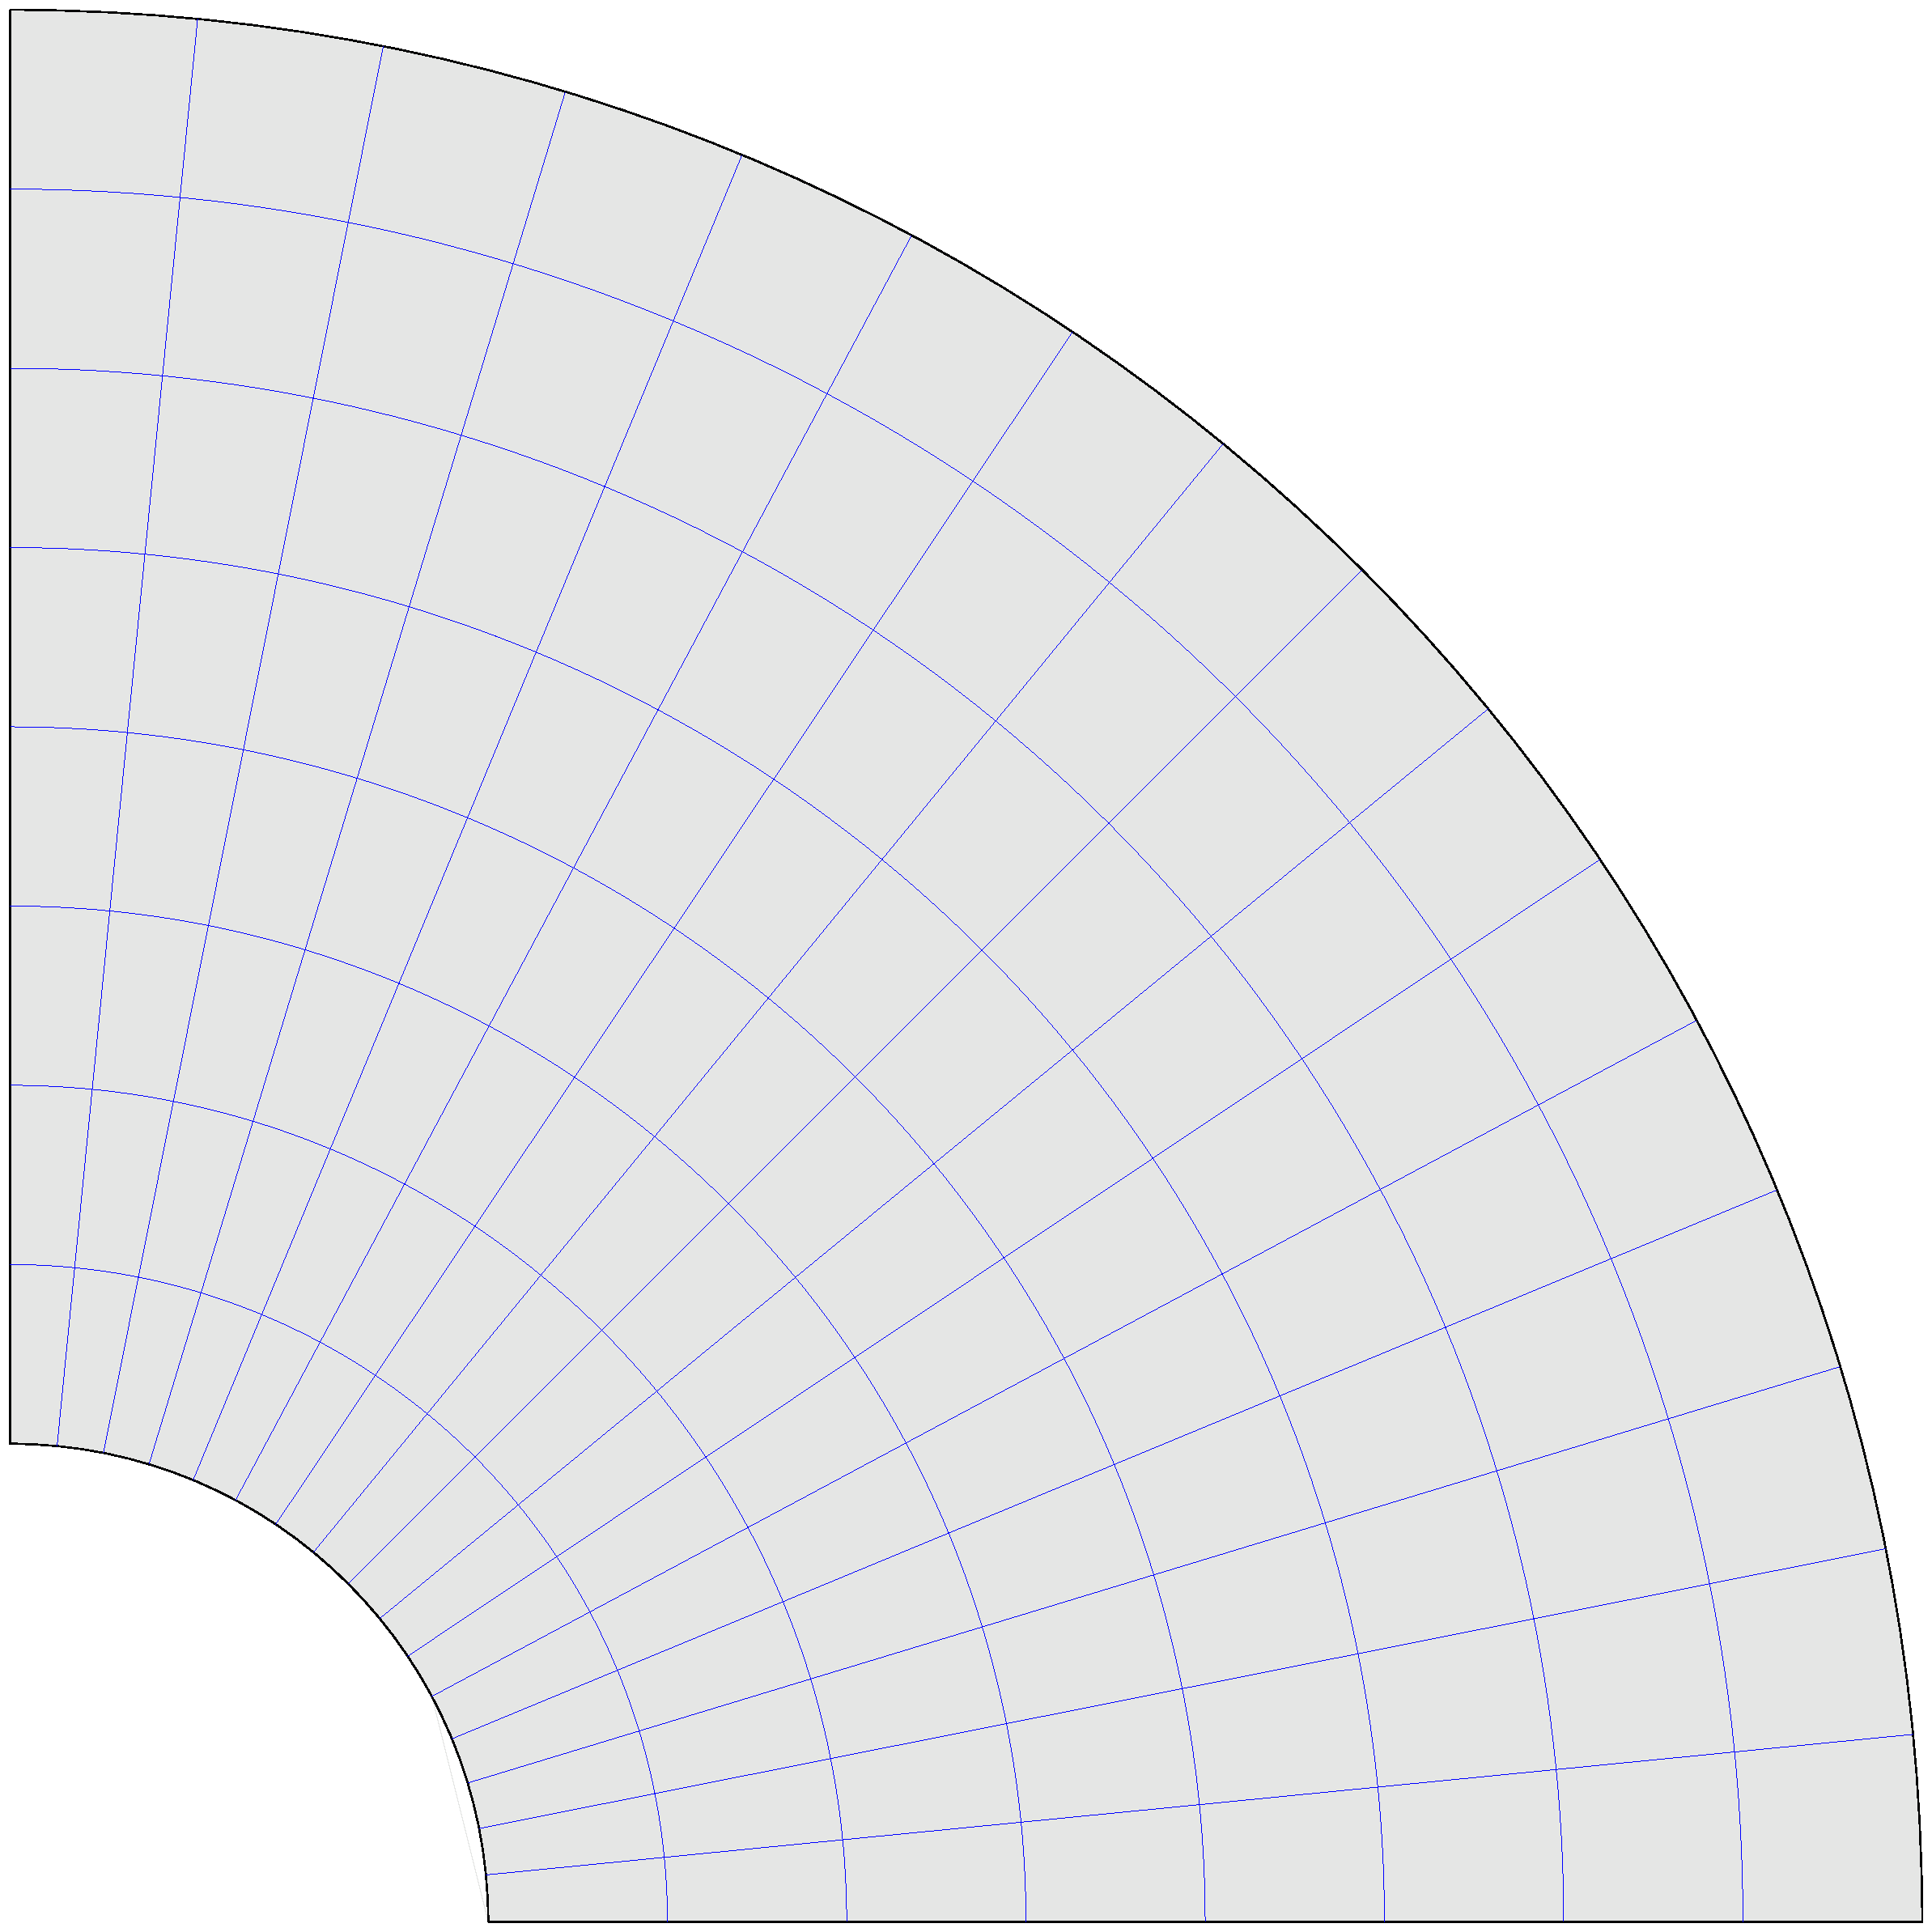
\includegraphics[width=\linewidth]{mesh_hole_3}
    \end{subfigure}
    \begin{subfigure}[b]{0.18\linewidth}        %% or \columnwidth
        \centering
        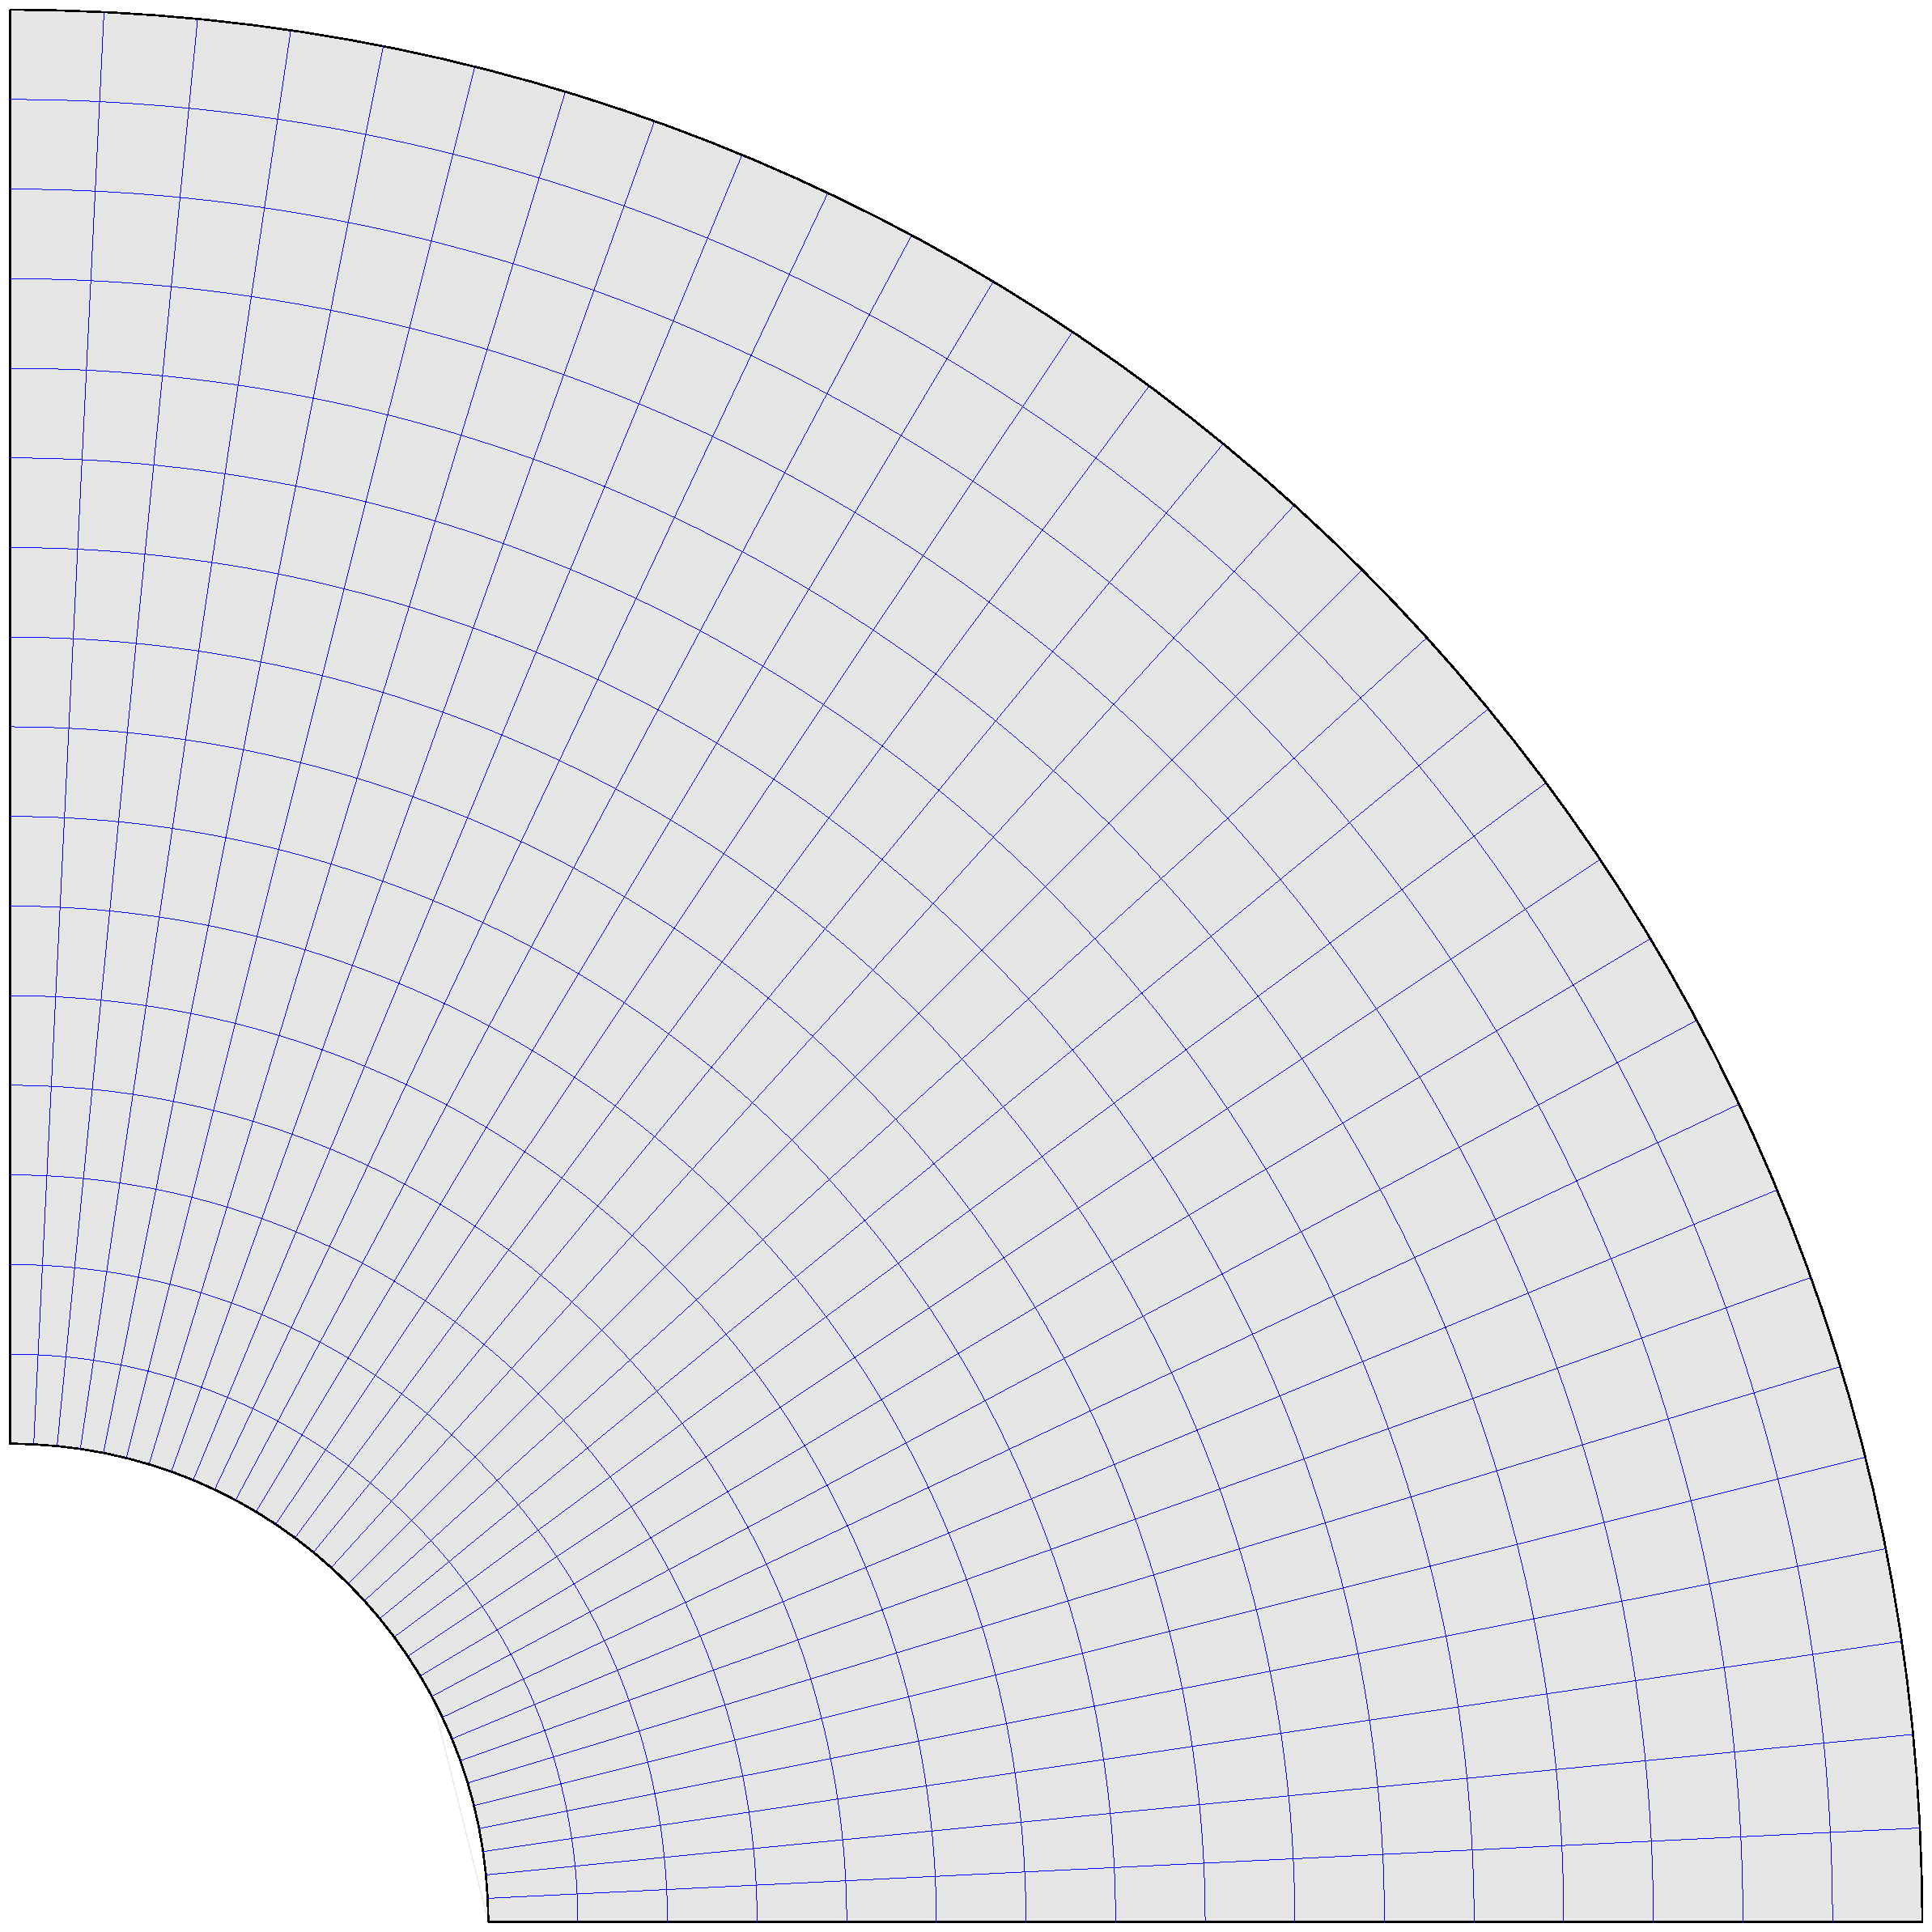
\includegraphics[width=\linewidth]{mesh_hole_4}
    \end{subfigure}
    \caption{Sequence of meshes for inf-sup test.}
    \label{fig:mesh_hole}
\end{figure}


Only the global $\bar{B}$ method and the non-symmetric \Bezier $\bar{B}$ method are considered here, as the symmetric \Bezier $\bar{B}$ method lacks a connection to a mixed formulation. As a counter example, the well-known pair $Q_p/Q_p$ of the global $\bar{B}$ method that violates the inf-sup condition is also tested here. Our tests follow the procedure proposed by Chapelle and Bathe in \cite{chapelle_inf-sup_1993}.\par
\begin{figure}[htb!]
    \centering
    \begin{subfigure}[b]{0.31\linewidth}        %% or \columnwidth
        \centering
        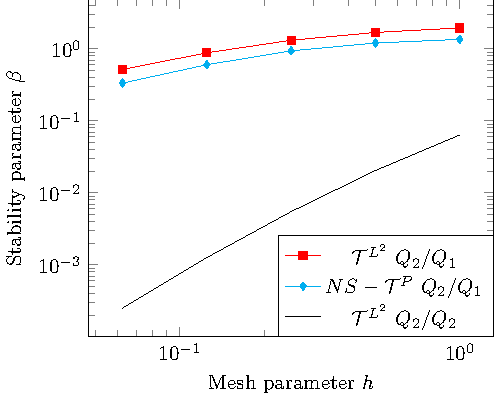
\includegraphics[width=\linewidth]{beta_p_2}
    \end{subfigure}
    \begin{subfigure}[b]{0.31\linewidth}        %% or \columnwidth
        \centering
        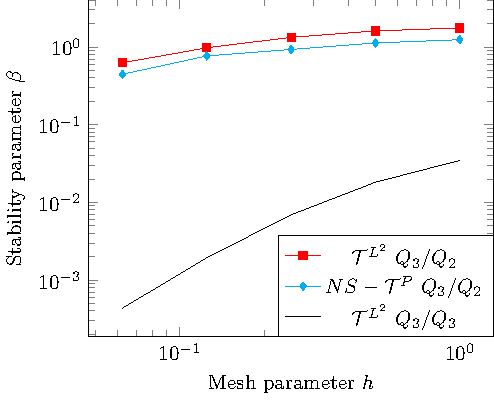
\includegraphics[width=\linewidth]{beta_p_3}
    \end{subfigure}
    \begin{subfigure}[b]{0.31\linewidth}        %% or \columnwidth
        \centering
        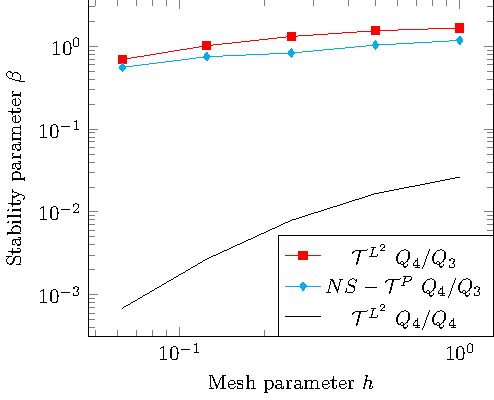
\includegraphics[width=\linewidth]{beta_p_4}
    \end{subfigure}

    \caption{Inf-sup test results for nearly incompressible elasticity. The global $\bar{B}$ method, $\mathcal{T}^{L^2} Q4/Q3$, and the non-symmetric \Bezier $\bar{B}$ method, $NS - \mathcal{T}^P Q4/Q3$, do not strictly satisfy the LBB condition, but compared to the $\mathcal{T}^{L^2} Q_4/Q_4$ method, both methods reduce constraints to a favorable level. }
    \label{fig:inf_sup}
\end{figure}

Figure \ref{fig:inf_sup} shows the numerical results. As can be seen, the global $\bar{B}$ method and the non-symmetric \Bezier $\bar{B}$ method do not strictly satisfy the LBB condition since $\beta$ is not independent of the mesh size. This result is consistent with the statement made in \cite{elguedj:hal-00457010} that the global $\bar{B}$ method does not reduce the constraints sufficiently to satisfy the LBB condition. However, compared to the $Q_p/Q_p$ pair, both methods reduce constraints to a more favorable level. If we compare the results for the global $\bar{B}$ method with the non-symmetric \Bezier $\bar{B}$ method we see that their stability parameter $\beta$ decreases at the same rate and the stability parameter for the non-symmetric \Bezier $\bar{B}$ method is slightly lower than that for the global $\bar{B}$ method. These results indicate a similar optimality in convergence for both methods and a slightly higher error for the non-symmetric \Bezier $\bar{B}$ method.

\subsubsection{Cook's membrane problem}

This benchmark problem is a standard test for combined bending and shearing response. The geometry, boundary conditions, and material properties are shown in Figure \ref{fig:Cook's}. The left boundary of the tapered panel is clamped, the top and bottom edges are free with zero traction boundary conditions, and the right boundary is subjected to a uniformly distributed traction load in the $y$-direction as shown. The meshes used are shown in Figure \ref{fig:mesh_cook}.
\begin{figure}[htb!]
	\centering
	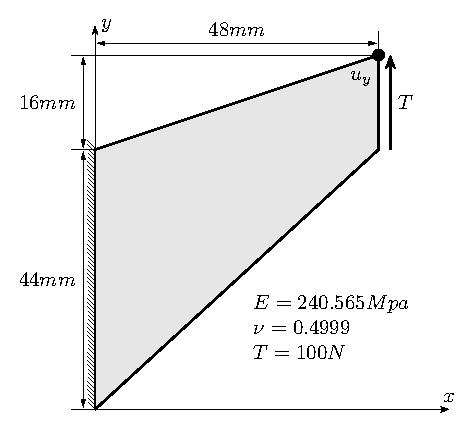
\includegraphics[width=0.5\linewidth]{Cook_s}
	\caption{Geometry, boundary conditions, and material properties for the Cook's membrane problem.}
	\label{fig:Cook's}
\end{figure}

A comparison of the displacement of the top right corner with respect to the number of elements per side is shown in Figure \ref{fig:Cook's_result}. $Q_1$ locks and mesh refinement has little impact. Locking is somewhat reduced for the higher-order elements $Q_p$, $p > 1$. The $\bar{B}$ methods perform very well for all degrees.
\begin{figure}[htb!]
    \centering
    \begin{subfigure}[b]{0.18\linewidth}        %% or \columnwidth
        \centering
        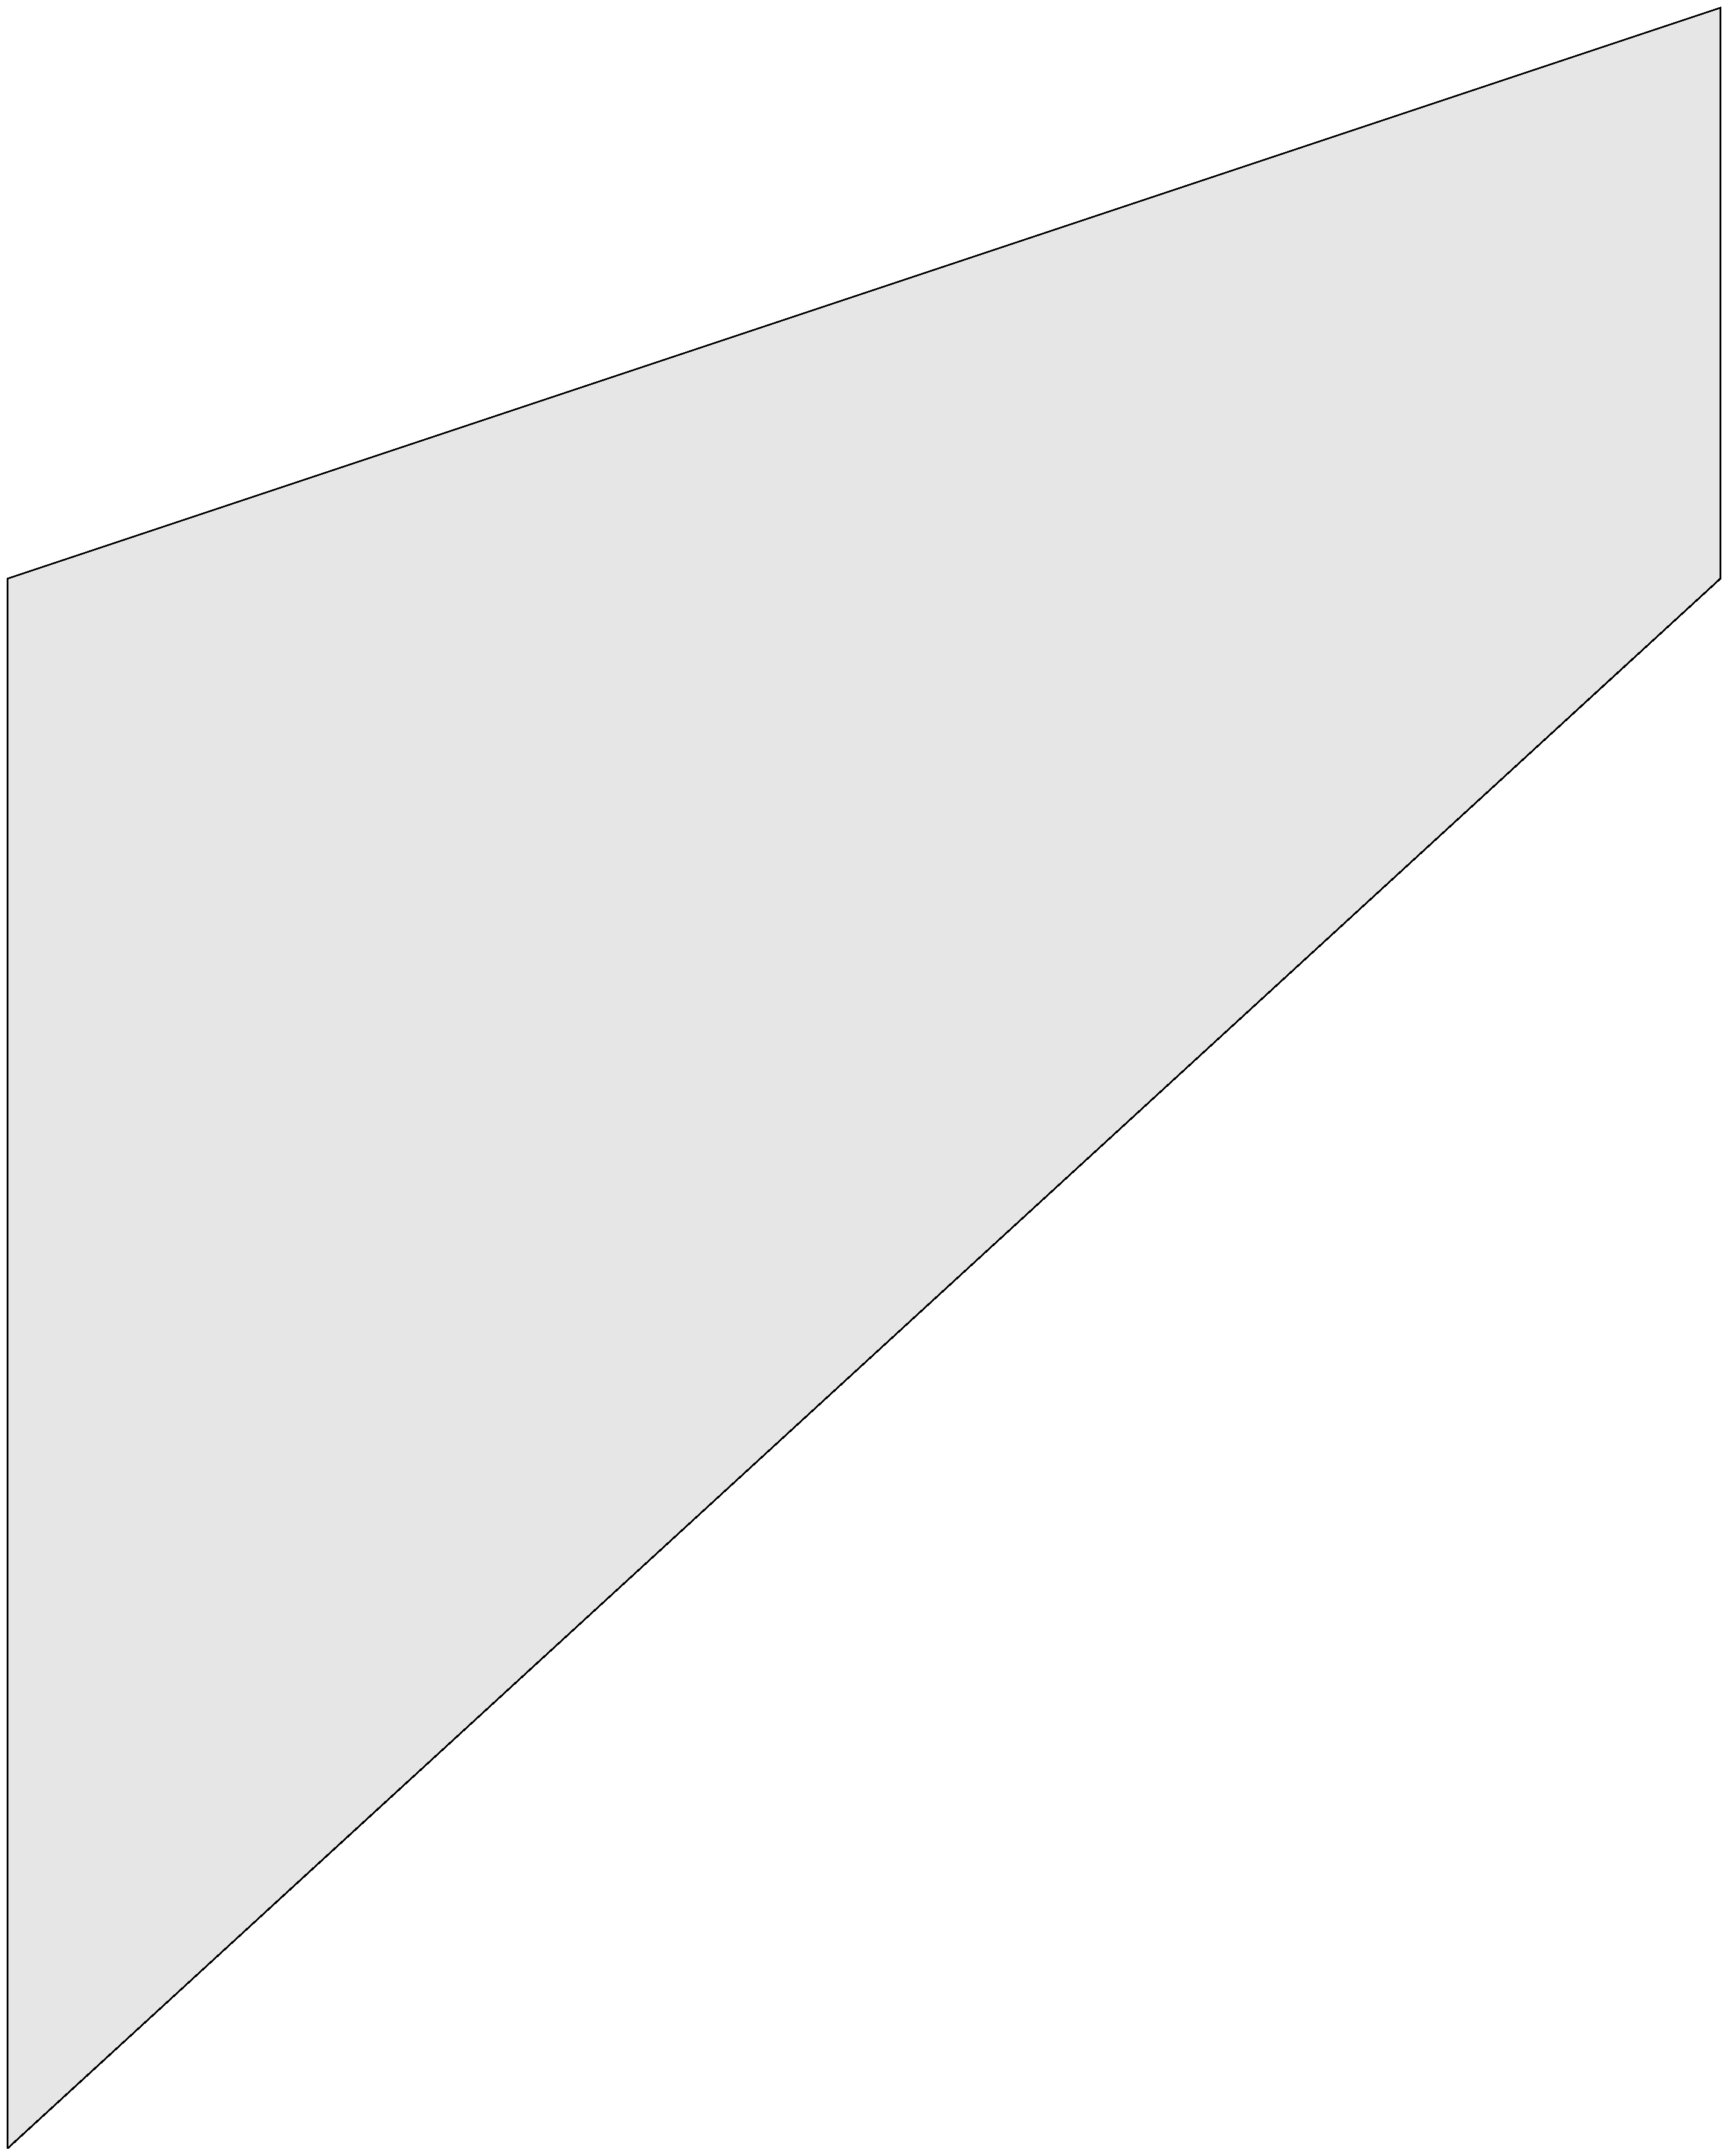
\includegraphics[width=\linewidth]{mesh_cook_0}
    \end{subfigure}
    \begin{subfigure}[b]{0.18\linewidth}        %% or \columnwidth
        \centering
        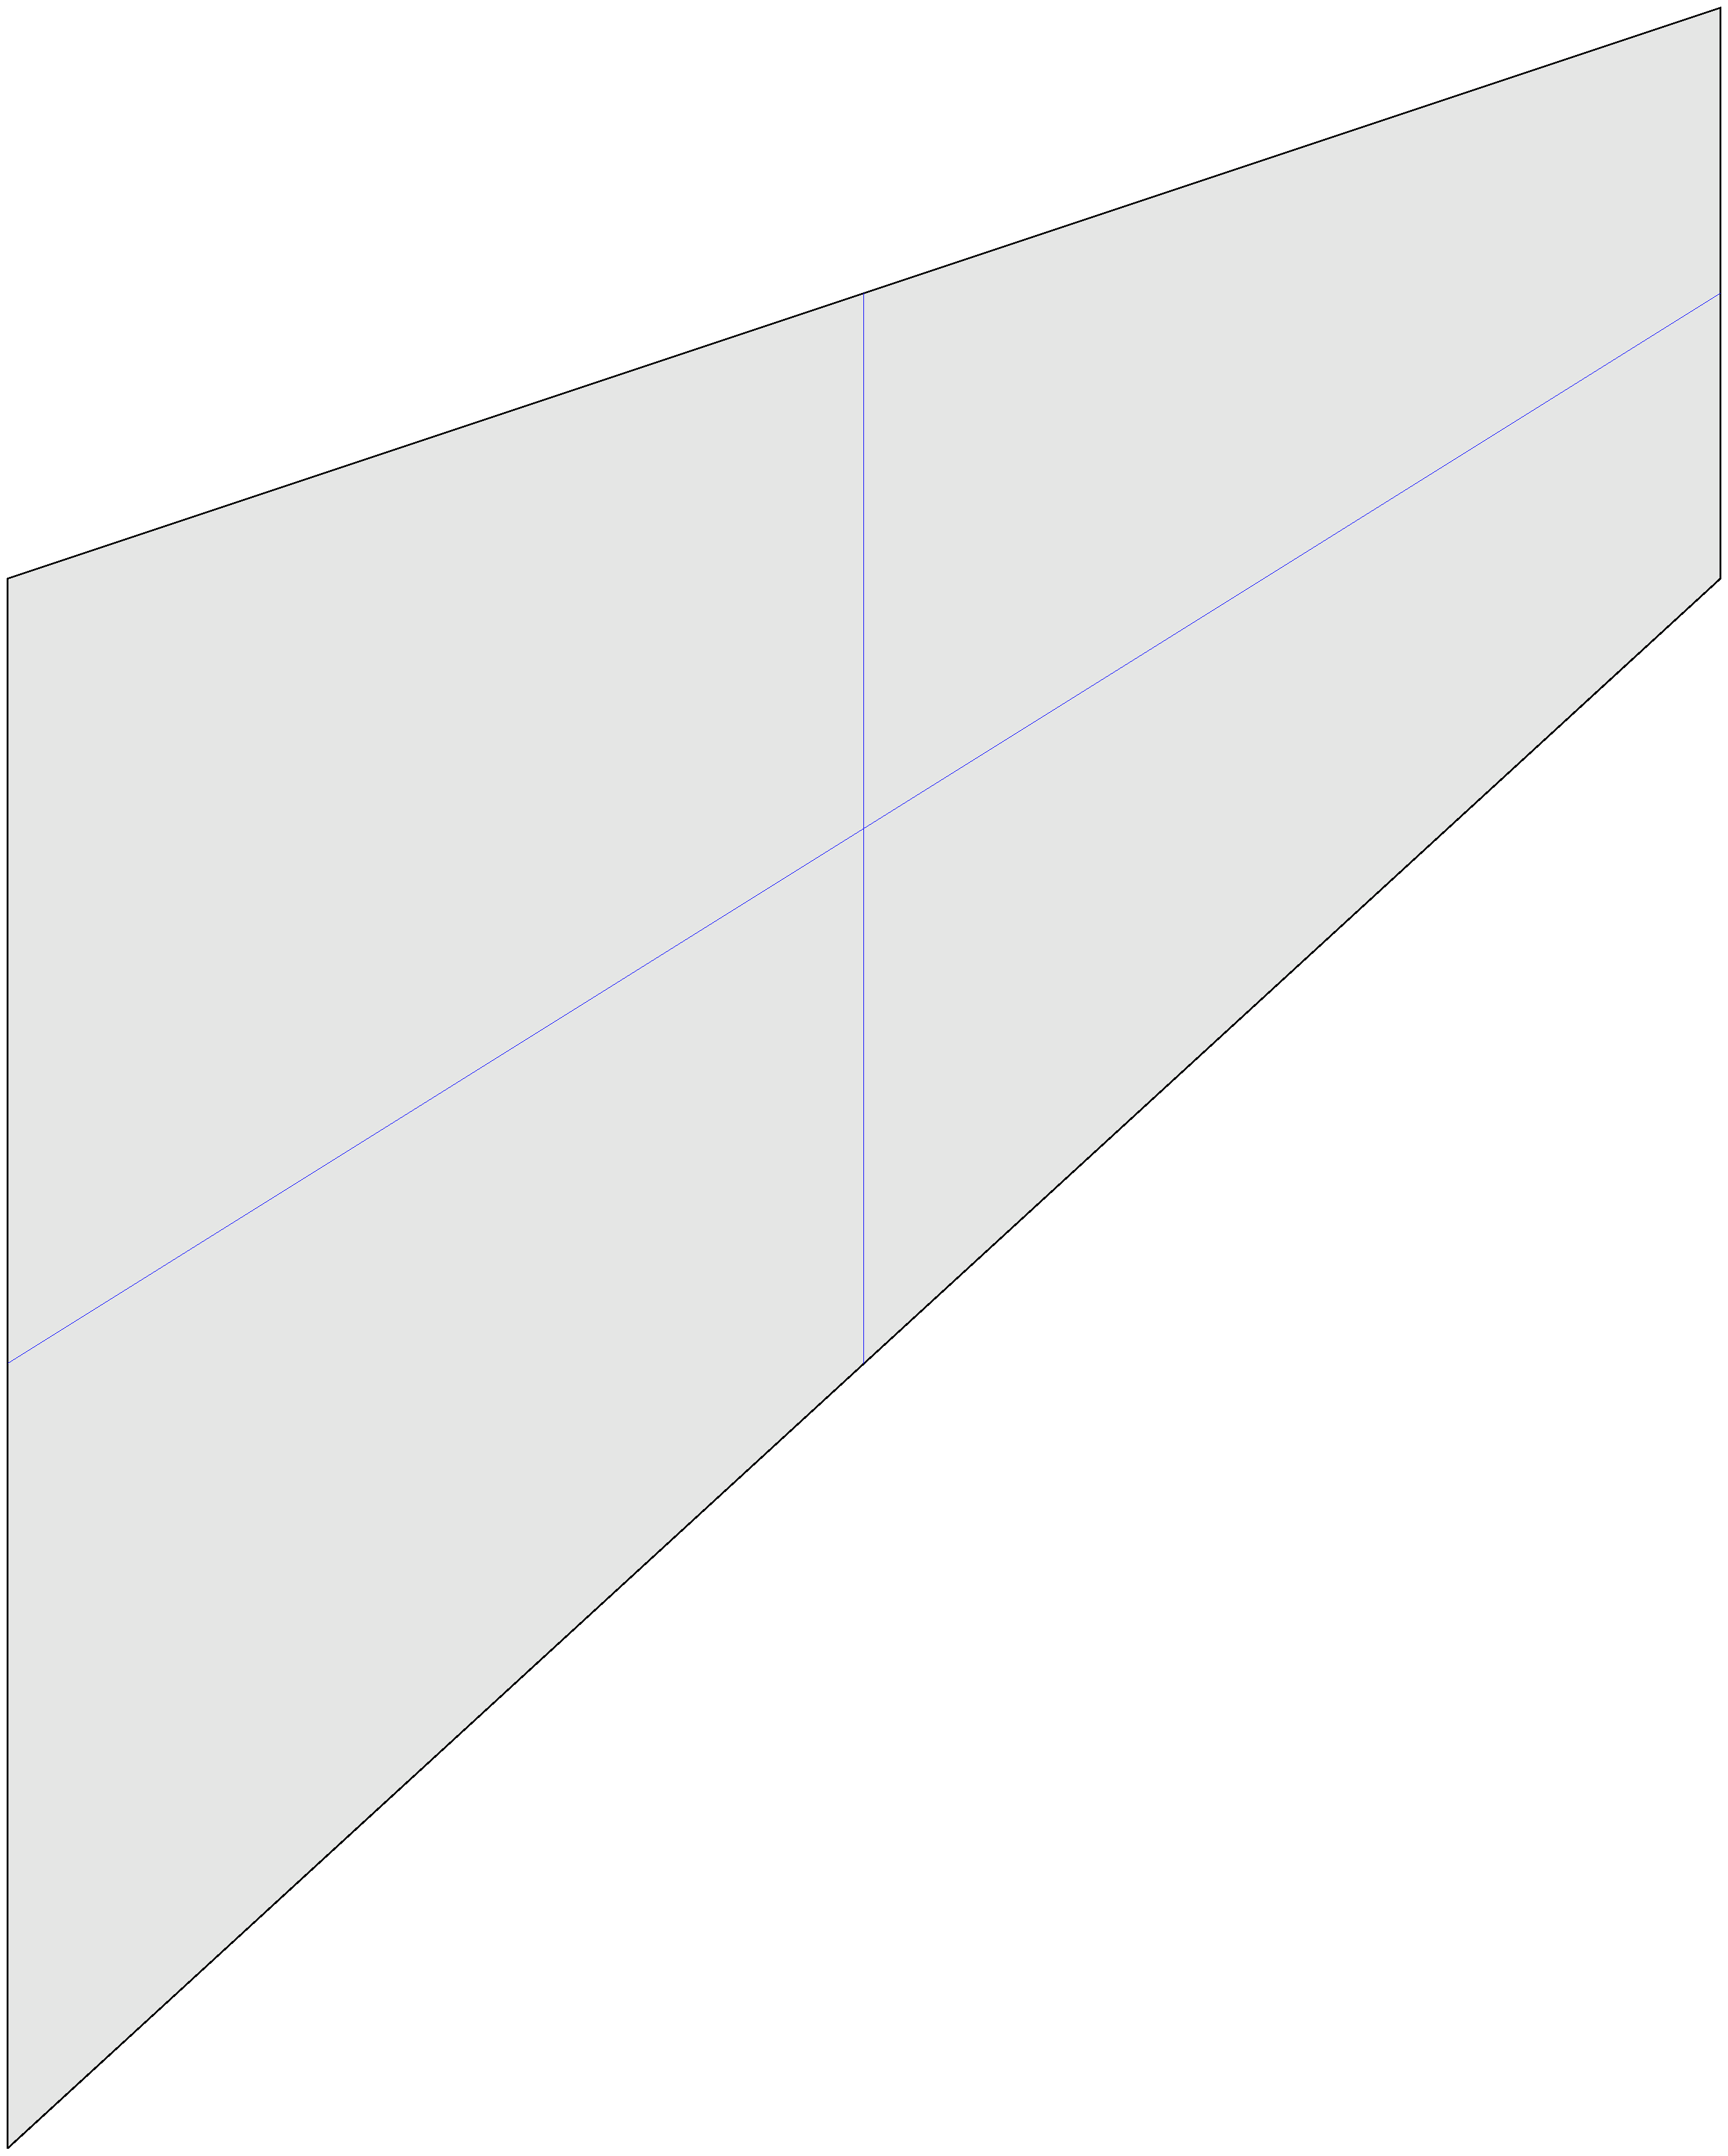
\includegraphics[width=\linewidth]{mesh_cook_1}
    \end{subfigure}
    \begin{subfigure}[b]{0.18\linewidth}        %% or \columnwidth
        \centering
        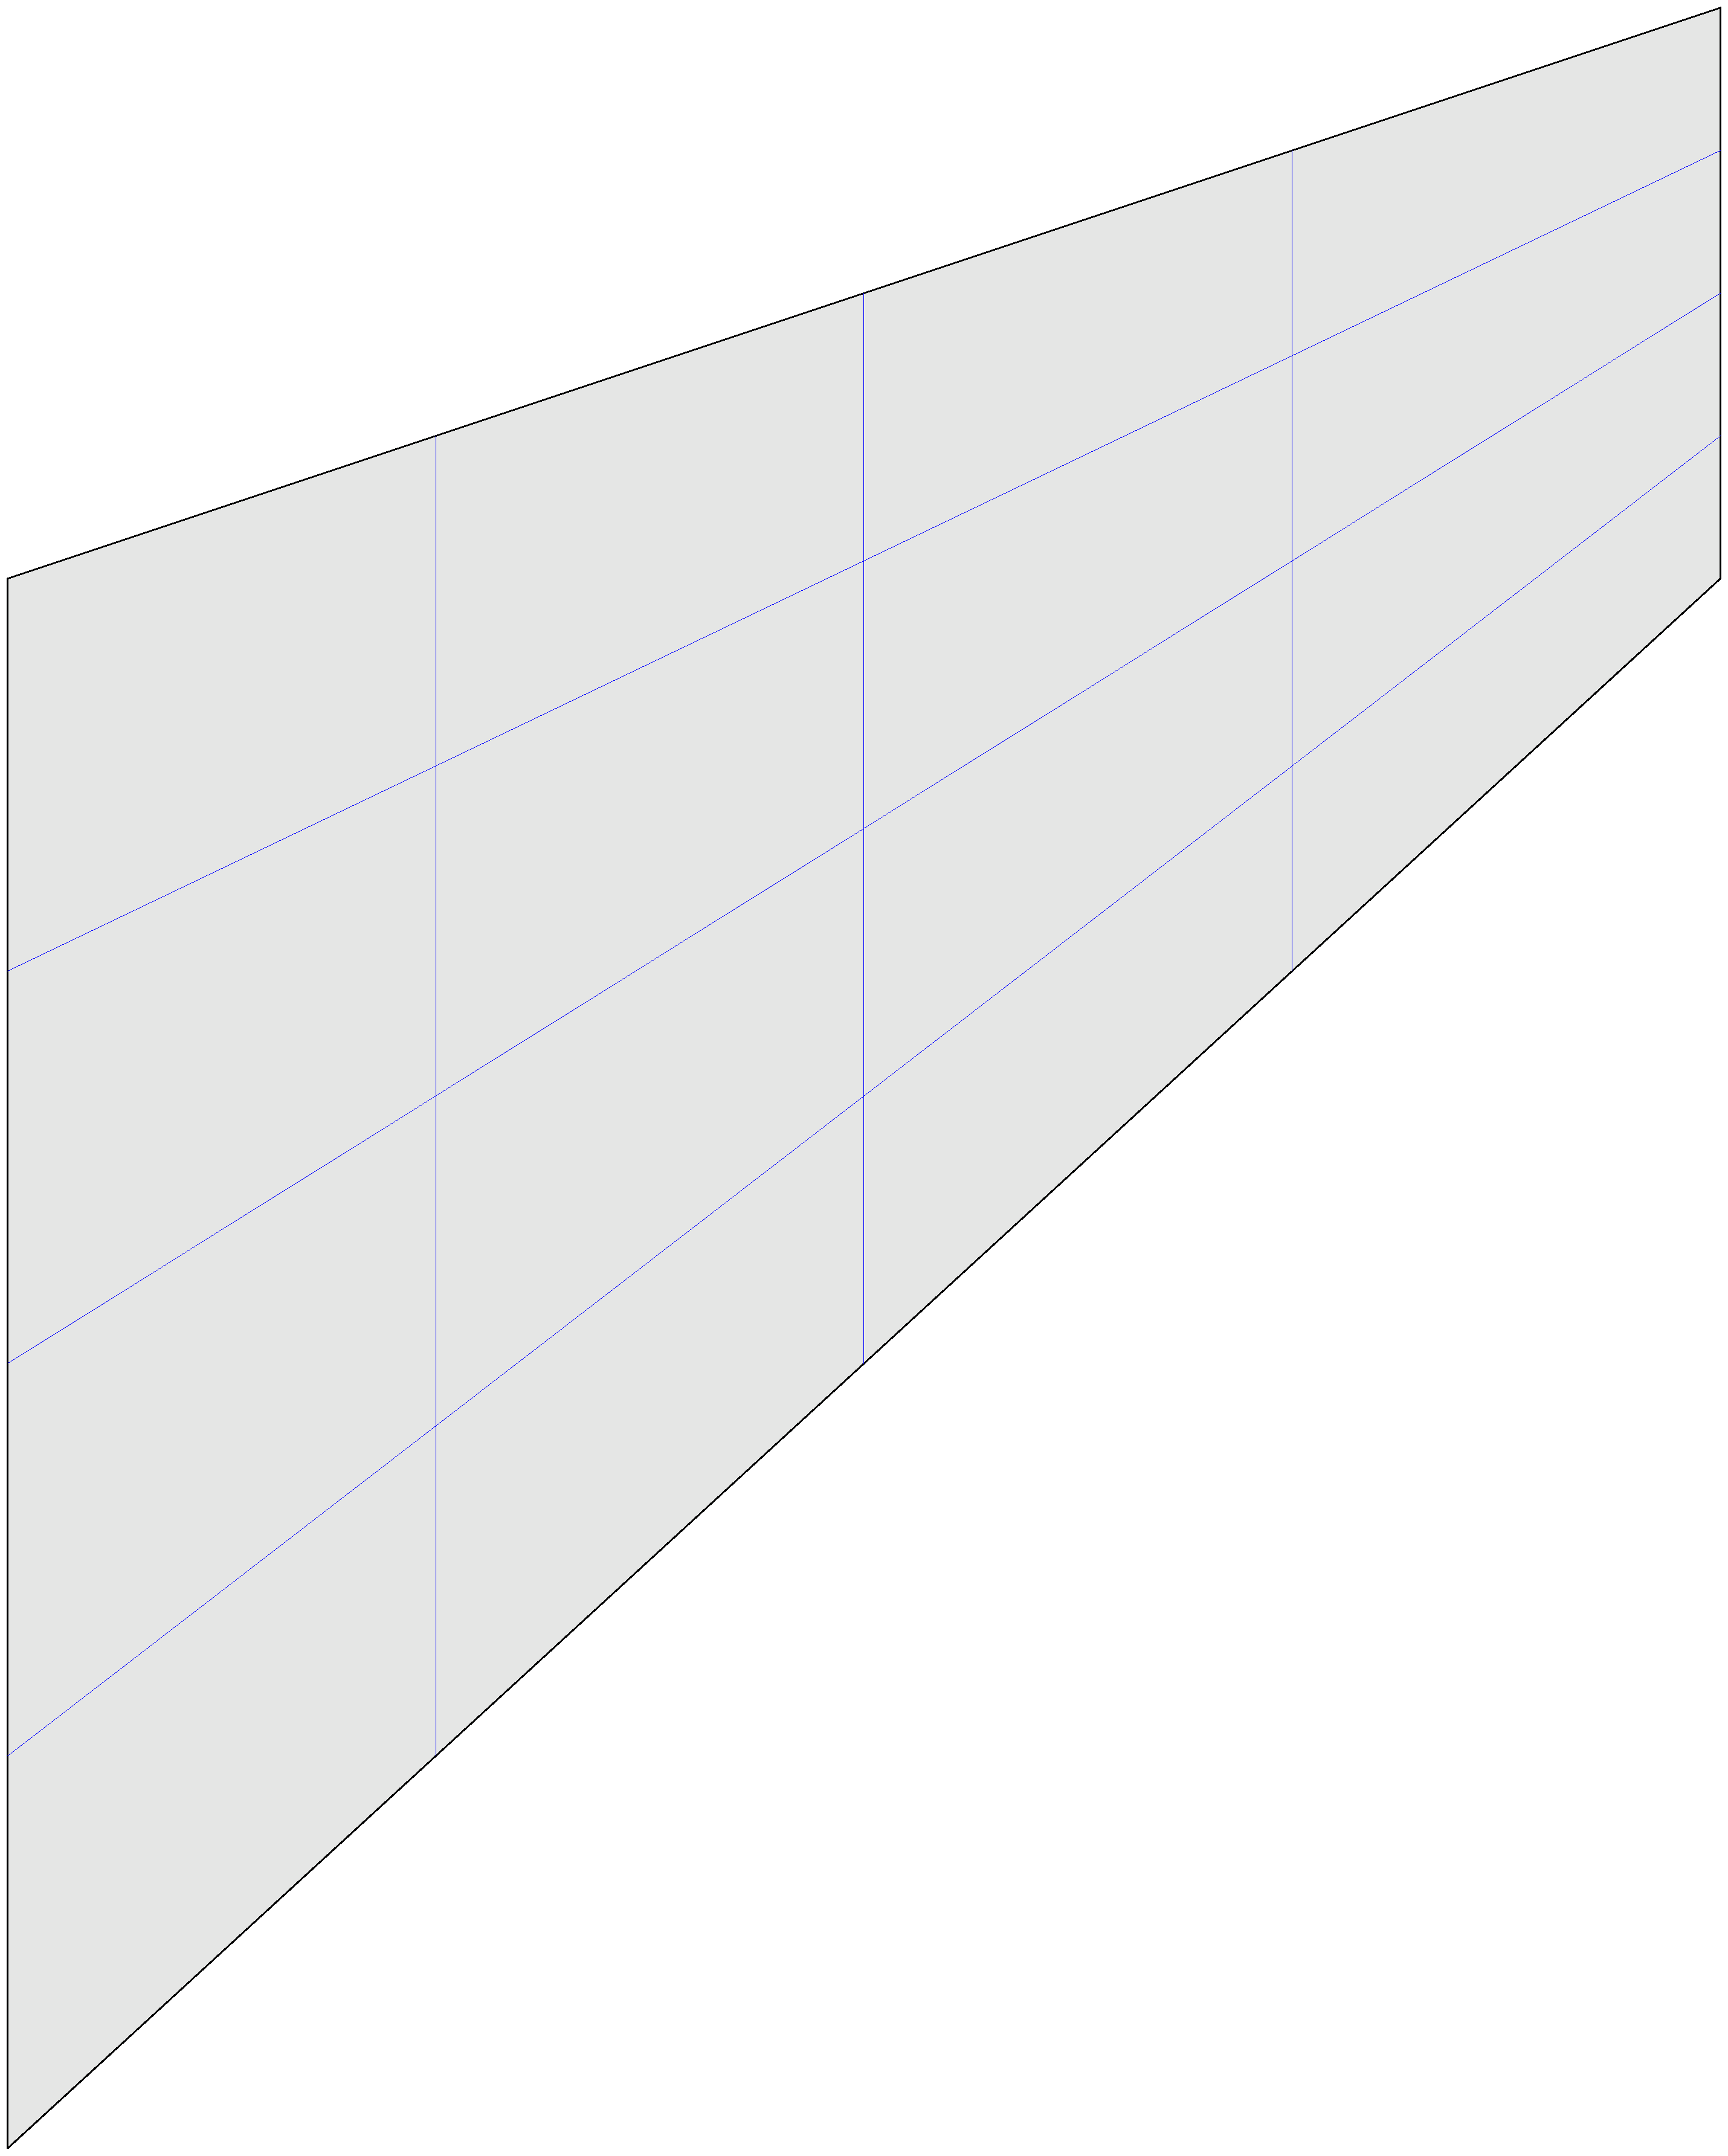
\includegraphics[width=\linewidth]{mesh_cook_2}
    \end{subfigure}
    \begin{subfigure}[b]{0.18\linewidth}        %% or \columnwidth
        \centering
        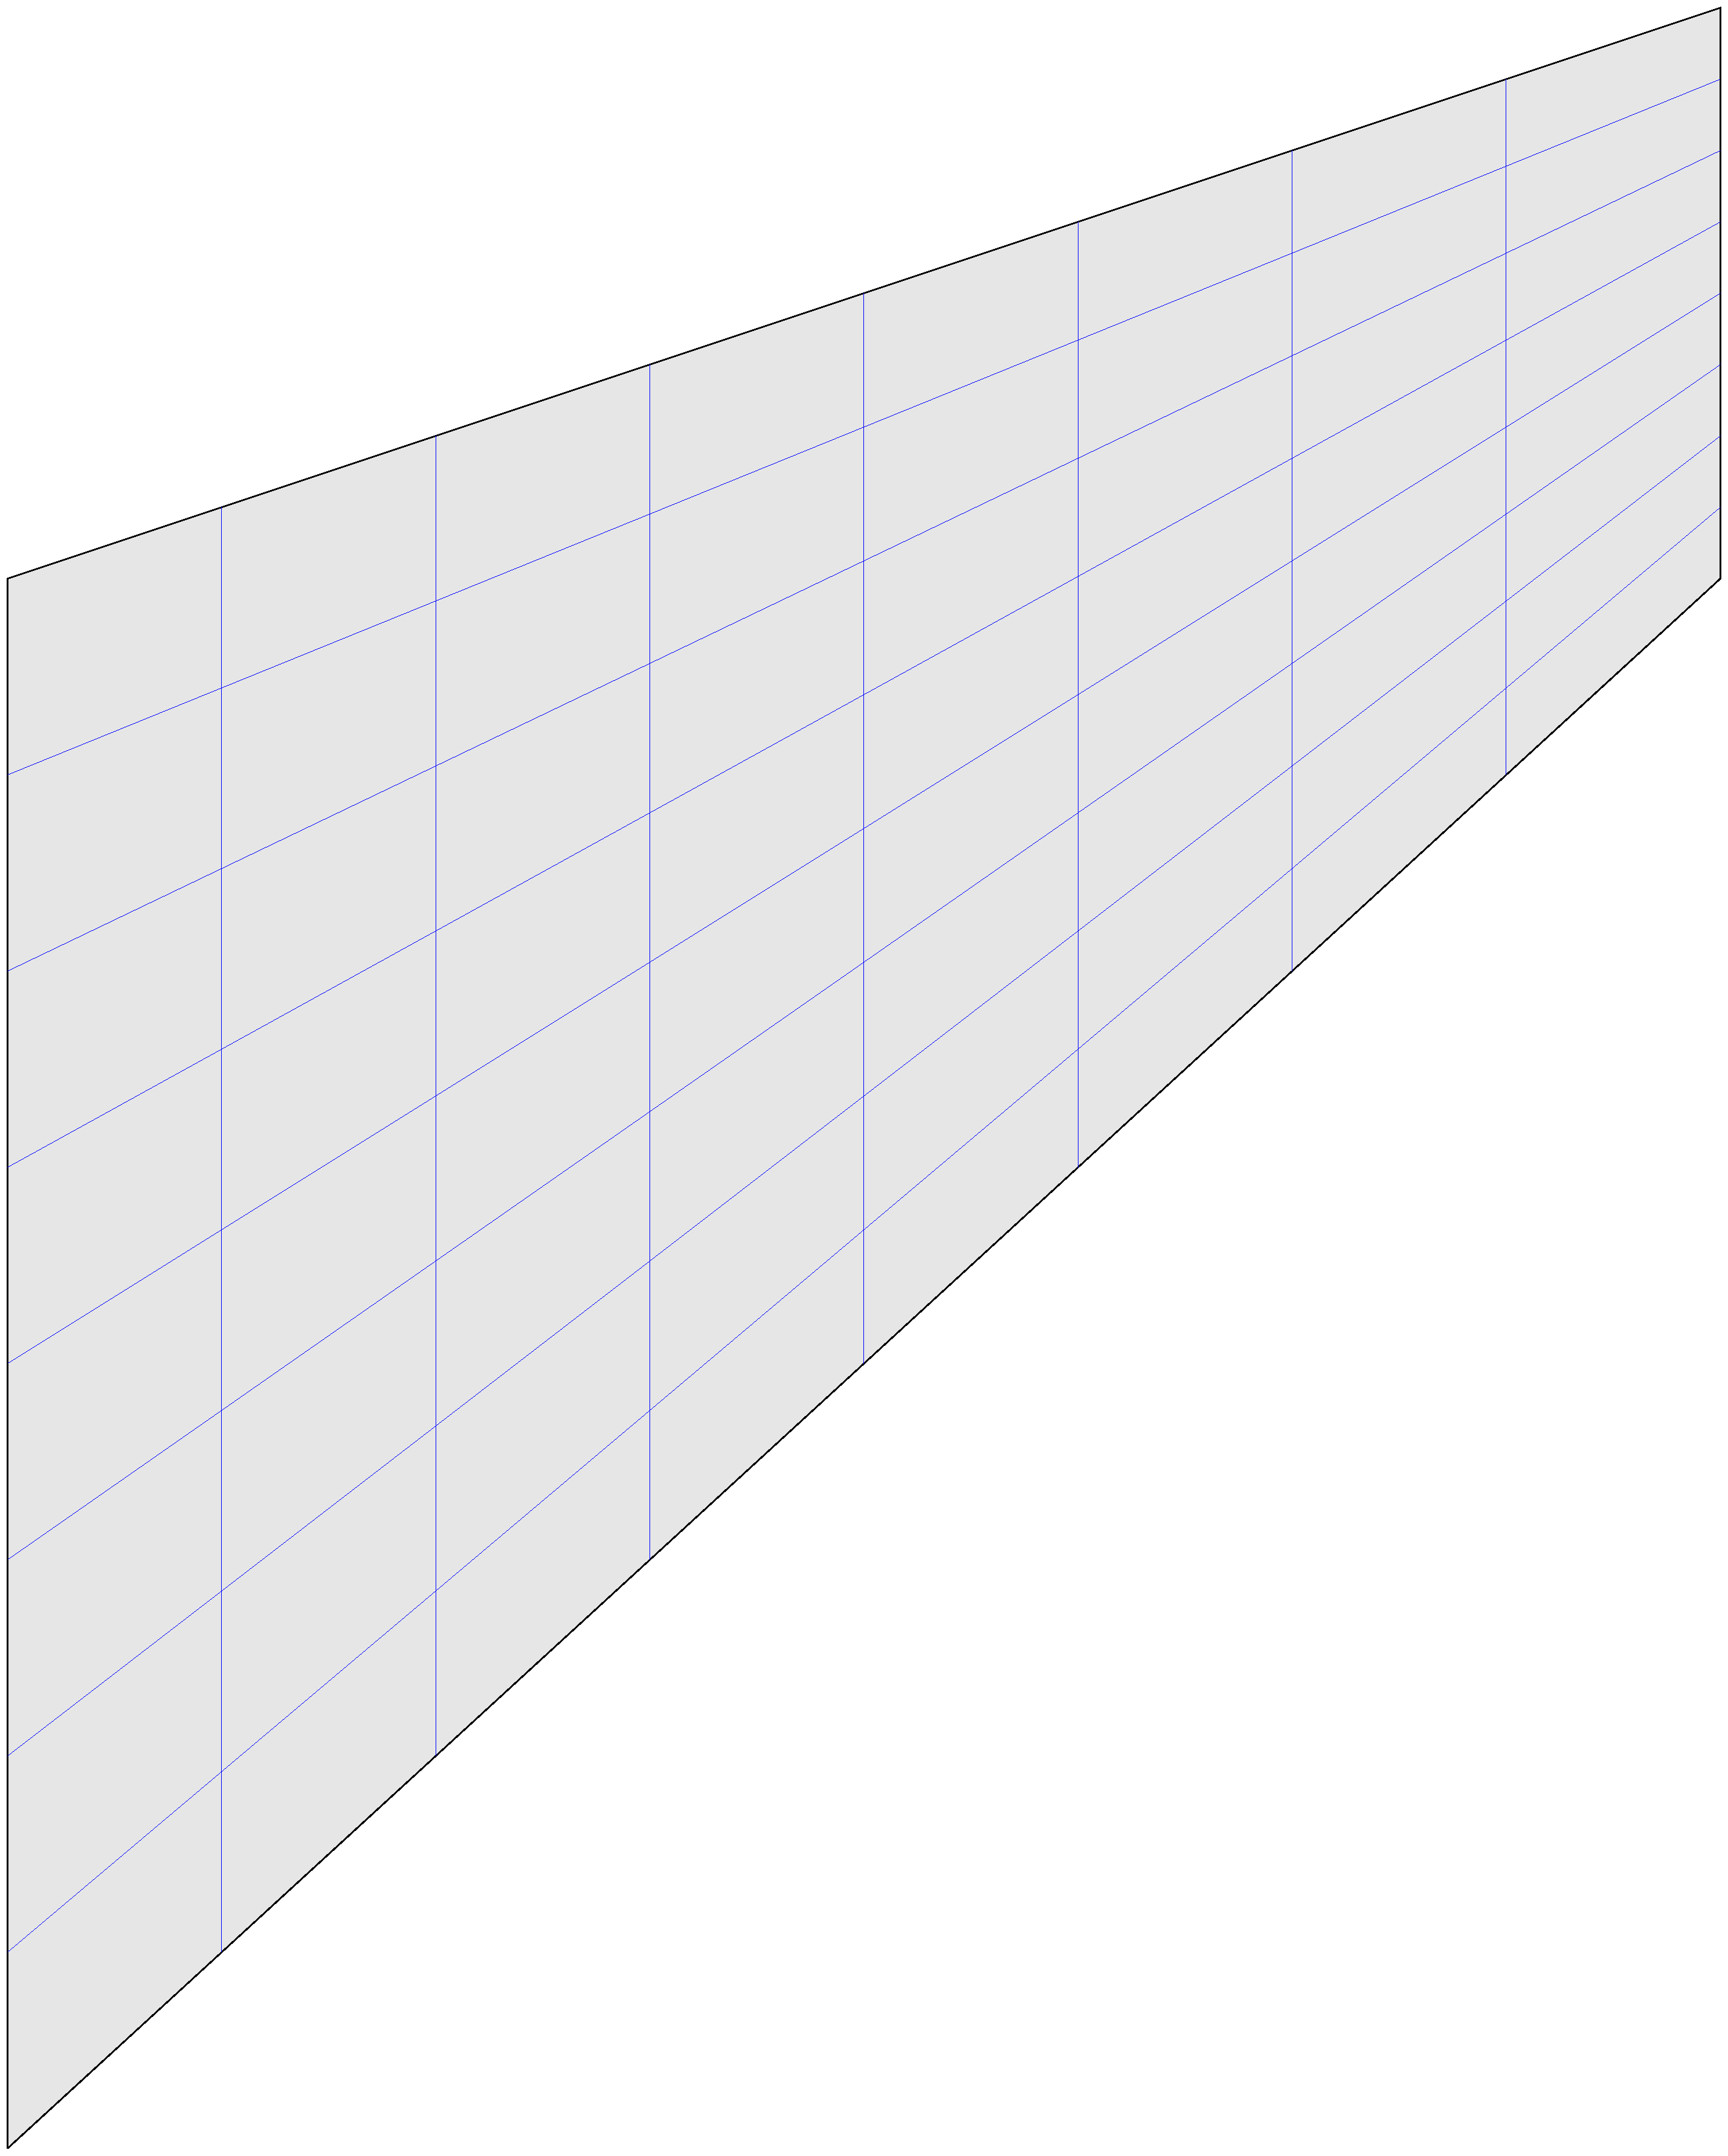
\includegraphics[width=\linewidth]{mesh_cook_3}
    \end{subfigure}
    \begin{subfigure}[b]{0.18\linewidth}        %% or \columnwidth
        \centering
        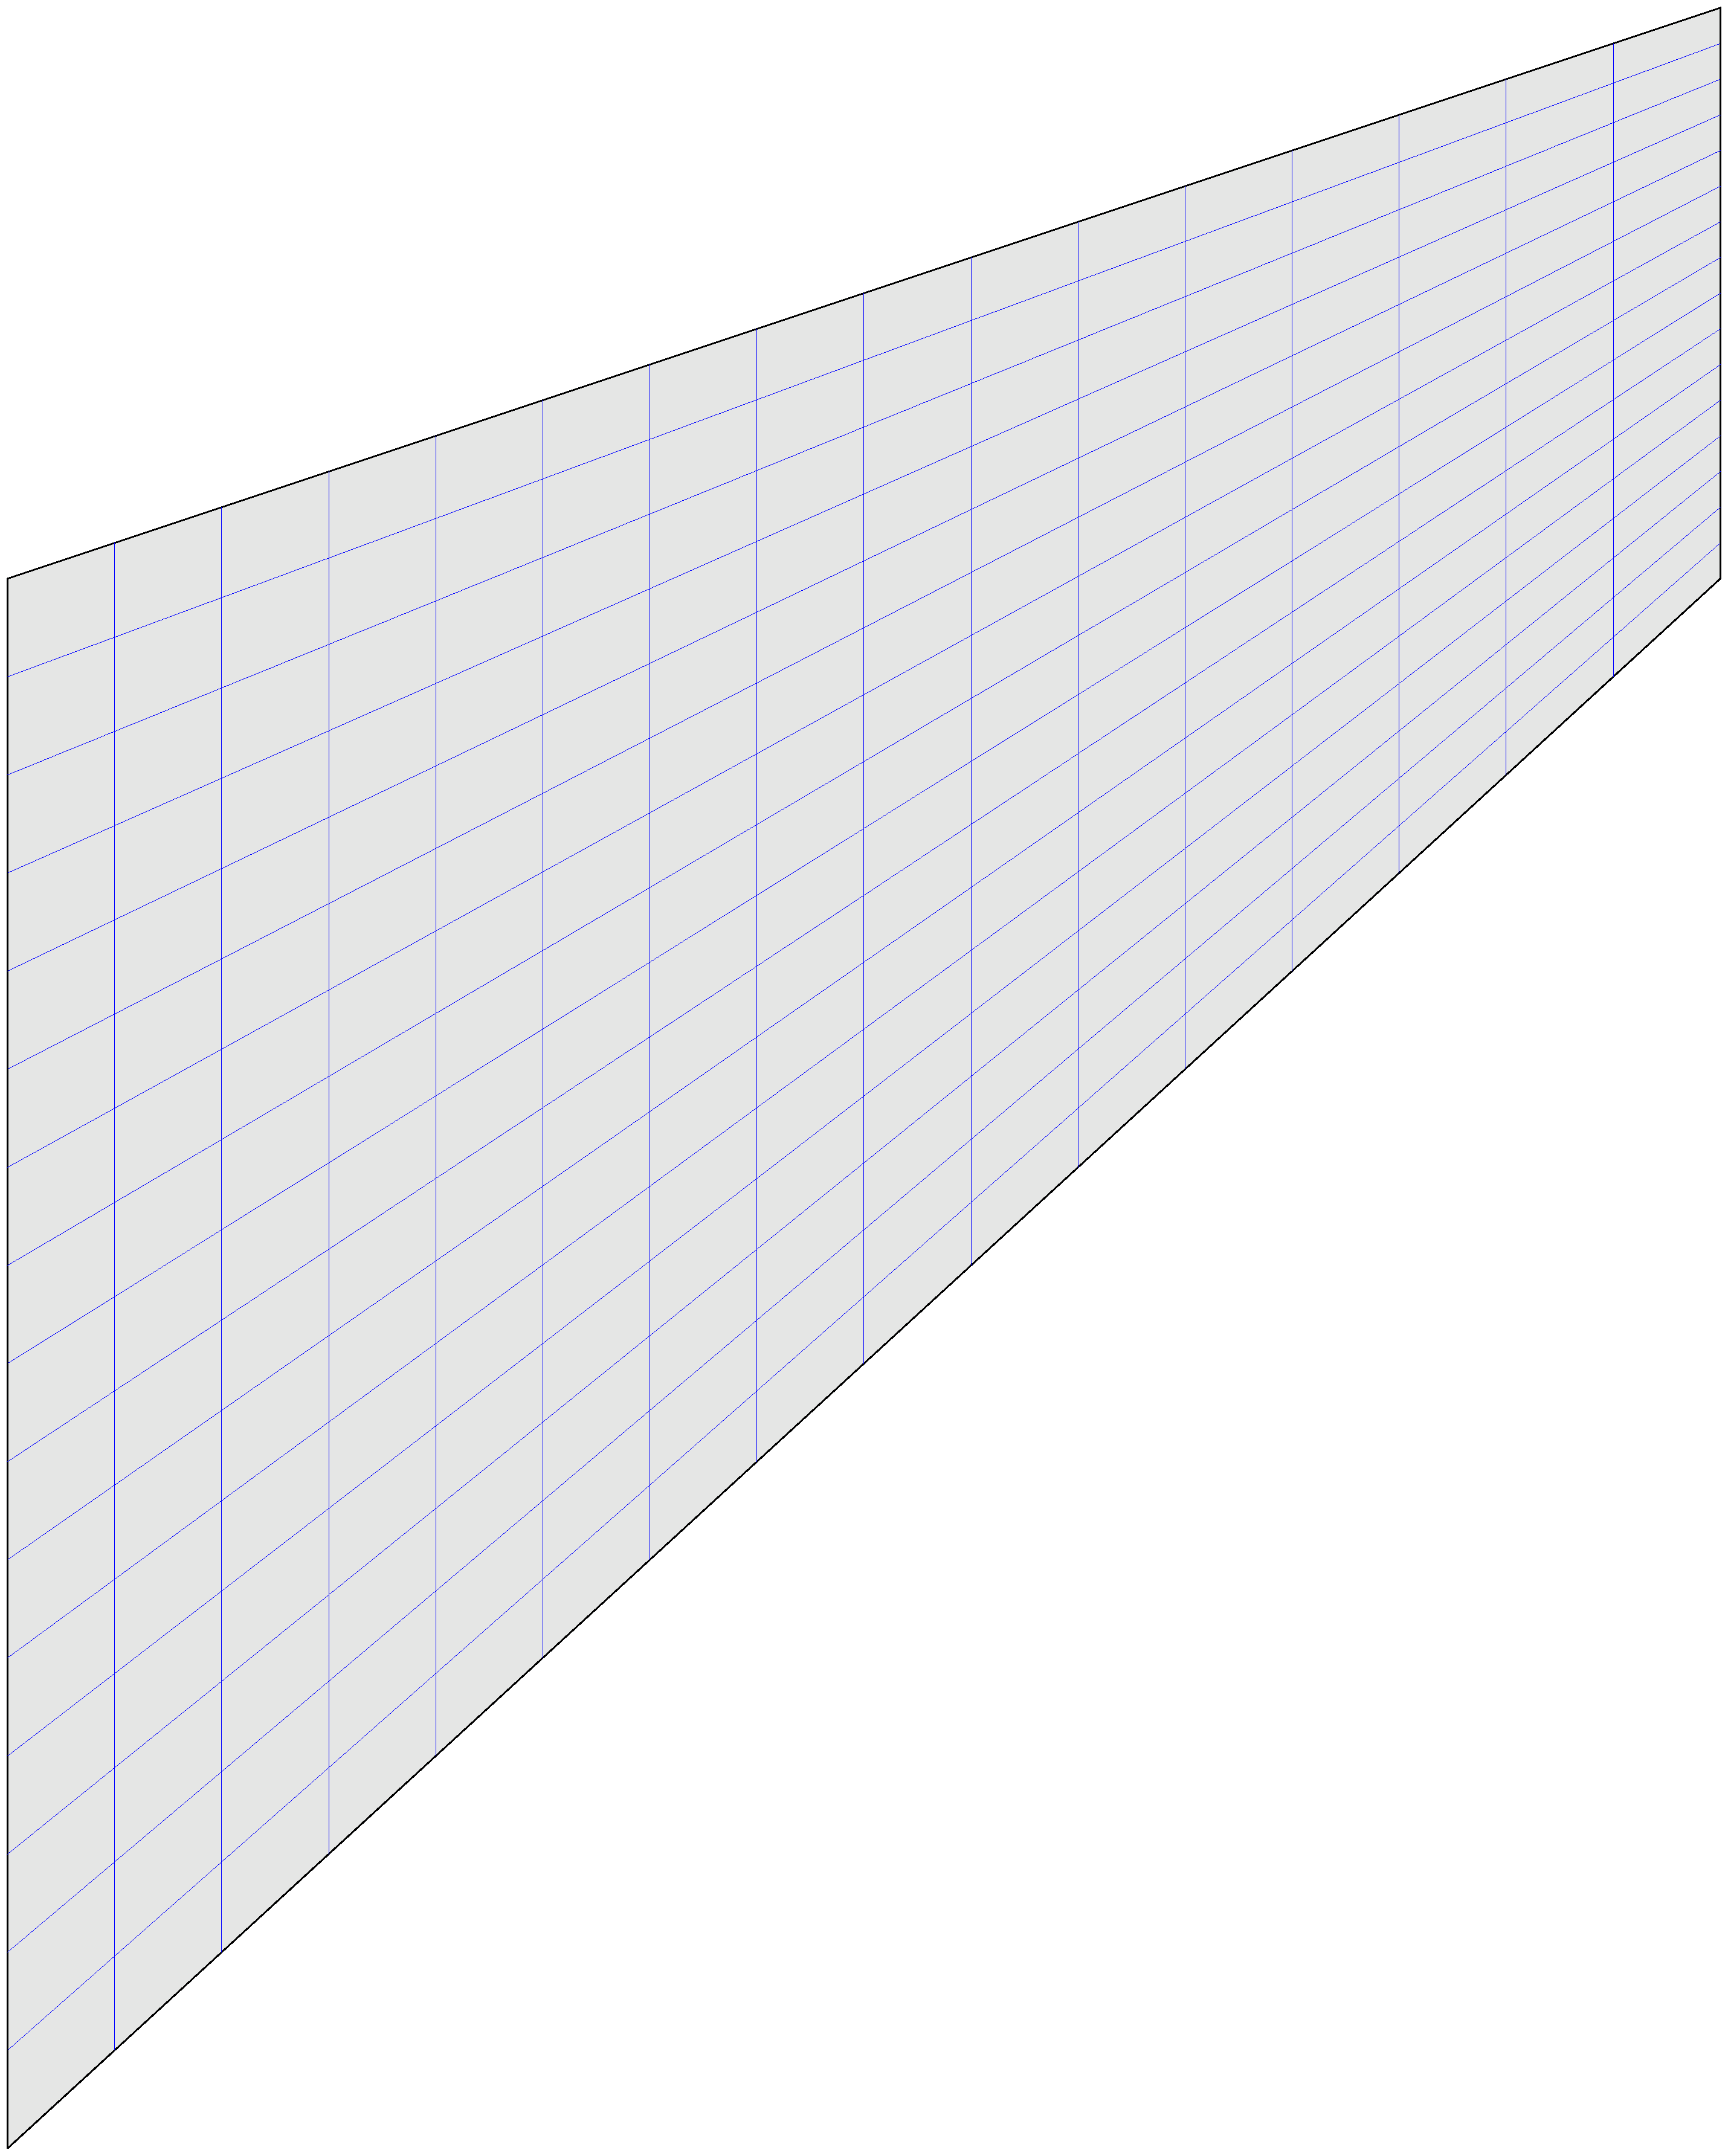
\includegraphics[width=\linewidth]{mesh_cook_4}
    \end{subfigure}
    \caption{Sequence of meshes for Cook's membrane problem.}
    \label{fig:mesh_cook}
\end{figure}

\begin{figure}[htb!]
    \centering
	\begin{subfigure}[b]{\textwidth}
        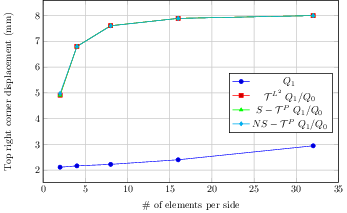
\includegraphics[width=.8\linewidth]{Cook's_membrane_Q1}
    \end{subfigure}
    %
    \centering
	\begin{subfigure}[b]{\textwidth}
        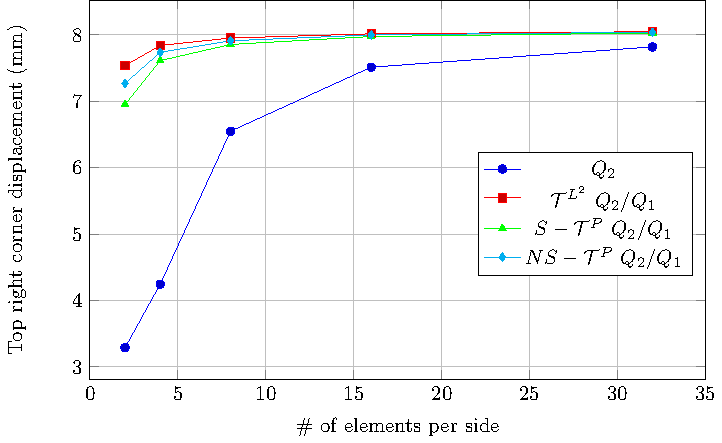
\includegraphics[width=.8\linewidth]{Cook's_membrane_Q2}
    \end{subfigure}
\end{figure}

\begin{figure}[htb!]\ContinuedFloat
    \centering
    \begin{subfigure}[b]{\textwidth}
        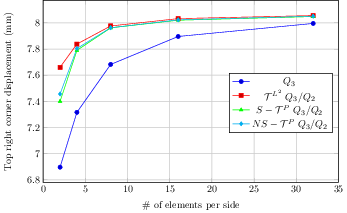
\includegraphics[width=.8\linewidth]{Cook's_membrane_Q3}
    \end{subfigure}
    %
    \centering
     \begin{subfigure}[b]{\textwidth}
        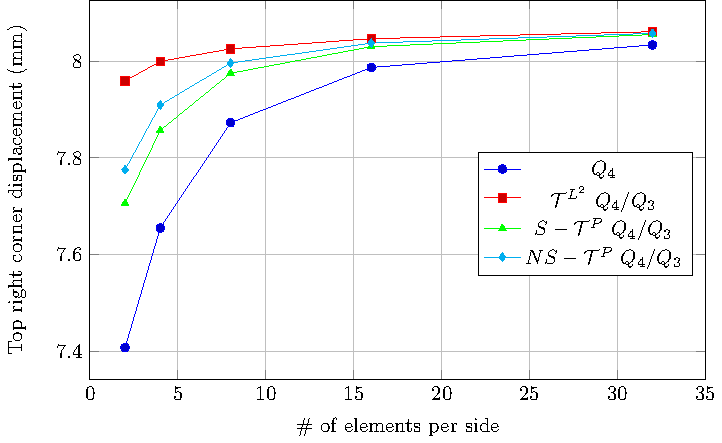
\includegraphics[width=.8\linewidth]{Cook's_membrane_Q4}
    \end{subfigure}
	\caption{Cook's membrane: comparison of the vertical displacement at the top right corner for the different methods and degrees.}
	\label{fig:Cook's_result}
\end{figure}

\clearpage

\subsubsection{Infinite plate with a circular hole}

The setup for the infinite plate with a circular hole problem is shown in Figure \ref{fig:platewithhole_geometry} and the discretizations are shown in Figure \ref{fig:mesh_hole}. The traction along the outer edge is evaluated from the exact solution which is given by
\begin{align}
\begin{split}
\sigma_{rr}(r,\theta)&=\dfrac{T_x}{2}(1-\dfrac{R_1^2}{r^2})+\dfrac{T_x}{2}(1-4\dfrac{R_1^2}{r^2}+3\dfrac{R_1^4}{r^4})cos(2\theta)\\
\sigma_{\theta\theta}(r,\theta)&=\dfrac{T_x}{2}(1+\dfrac{R_1^2}{r^2})-\dfrac{T_x}{2}(1+3\dfrac{R_1^4}{r^4})cos(2\theta)\\
\sigma_{r\theta}(r,\theta)&=-\dfrac{T_x}{2}(1+2\dfrac{R_1^2}{r^2}-3\dfrac{R_1^4}{r^4})sin(2\theta).
\end{split}
\end{align}
\begin{figure}[htb!]
	\centering
	\begin{subfigure}[t]{0.5\textwidth}
    \centering
    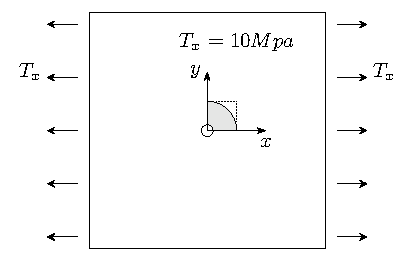
\includegraphics[width=1\linewidth]{Platewithhole}
    \caption{Infinite plate with a hole subjected to uniaxial tension at $x=\pm\infty$.}
    \label{fig:platewithhole_geometry_a}
    \end{subfigure}%
    ~ 
    \begin{subfigure}[t]{0.5\textwidth}
    \centering
    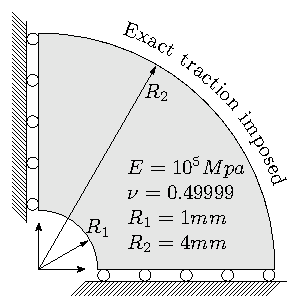
\includegraphics[width=1\linewidth]{Platewithhole_b}
    \caption{A representation of the computational model.}
    \label{fig:platewithhole_geometry_b}
    \end{subfigure}
    \caption{Geometry, boundary conditions, and material properties for the infinite plate with a hole.}
	\label{fig:platewithhole_geometry}
\end{figure}

Convergence plots for the relative error of the displacement and energy in the $L^2$ norm are shown in Figure \ref{fig:platewithhole_convergence}. As can be seen, the standard $Q_p$ approximations suffer from severe volumetric locking for all orders while, on the other hand, the $\bar{B}$ methods remedy locking for all cases. {For the symmetric \Bezier $\bar{B}$ method, optimal rates are achieved in all three measures for biquadratic elements and the optimal energy convergence has been achieved for bicubic elements, but convergence has degraded in all three measures for the biquartic elements. This reduction in convergence rates results from the fact that the derivation of the symmetric \Bezier $\bar{B}$ method is purely based on the engineering analogy between the $L^2$ projection and \Bezier projection operations. The non-symmetric \Bezier $\bar{B}$ method, on the other hand, achieves optimal convergence in the displacement, stress, and energy norms for all elements with slightly higher errors than those of the global $\bar{B}$ method.}

{Contour plots of  $\sigma_{xx}$ from the finest biquartic discretization are shown in Figure \ref{fig:platewithhole_contour}. We can see that results from all $\bar{B}$ methods are consistent with the reference solution, but using the standard finite element approach results in meaningless stresses. Figure \ref{fig:platewithhole_error_contour} shows the absolute error of $\sigma_{xx}$ from the same discretization. We can see that the projection methods produce an error of less than $.1\%$ of the maximum $\sigma_{xx}$, while the error for the standard $Q_4$ element is of the same order as the maximum $\sigma_{xx}$. We can also see that the non-symmetric method provides a slight improvement when compared to the symmetric method.}
\begin{figure}[h]
    \center
\begin{tabular}{ccc}
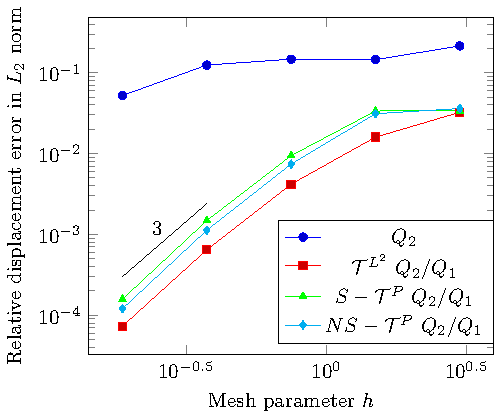
\includegraphics[width=.31\linewidth]{deformation_p_2} & 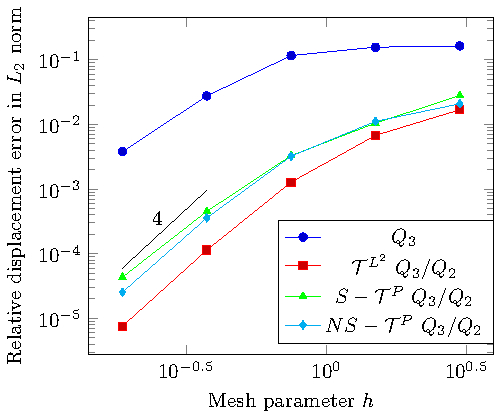
\includegraphics[width=.31\linewidth]{deformation_p_3} & 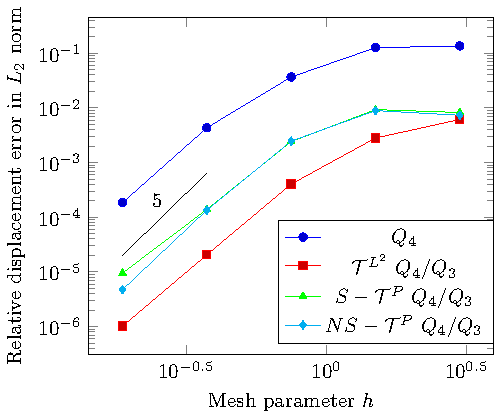
\includegraphics[width=.31\linewidth]{deformation_p_4}\\
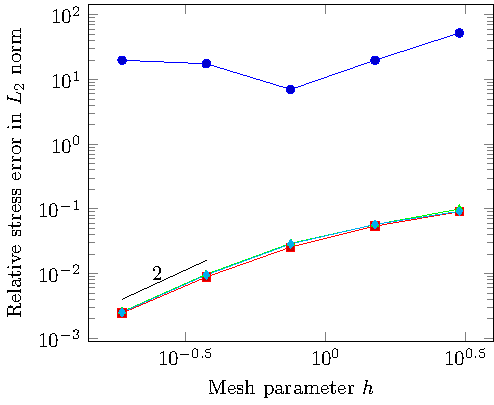
\includegraphics[width=.31\linewidth]{stress_p_2} & 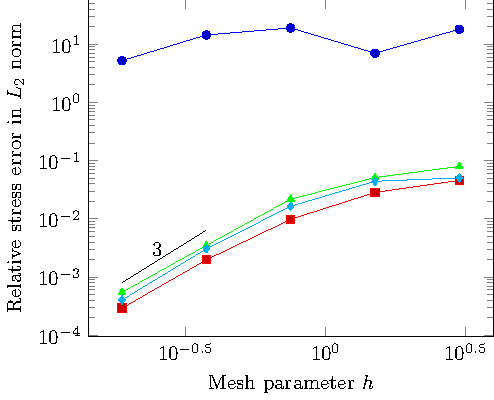
\includegraphics[width=.31\linewidth]{stress_p_3} & 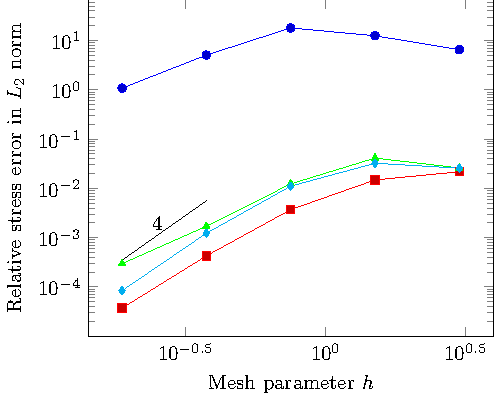
\includegraphics[width=.31\linewidth]{stress_p_4}\\
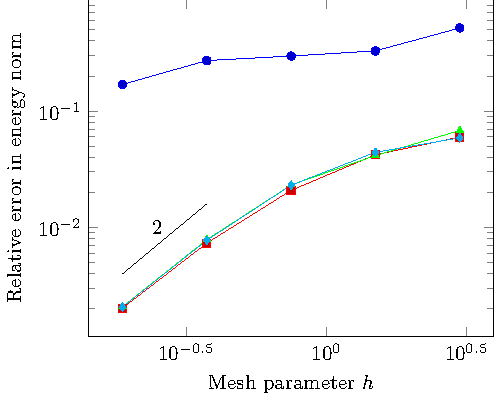
\includegraphics[width=.31\linewidth]{energy_p_2} & 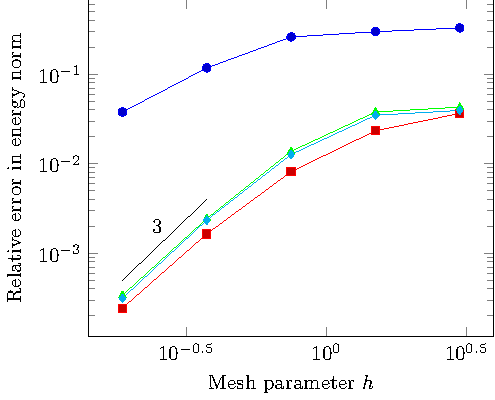
\includegraphics[width=.31\linewidth]{energy_p_3} & 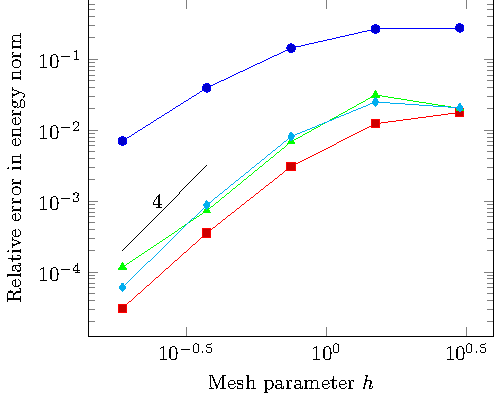
\includegraphics[width=.31\linewidth]{energy_p_4}
\end{tabular}
    \caption{Convergence study of the plate with a circular hole. The relative $L^2$ error of displacement, stress and the relative error in energy norm with respect to mesh refinement.}
	\label{fig:platewithhole_convergence}
\end{figure}


\begin{figure}[htb!]
    \center
    \begin{tabular}{cc}
    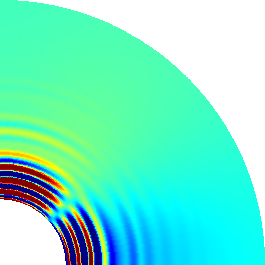
\includegraphics[width=.4\linewidth]{no_stress_contour} & 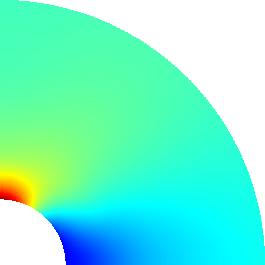
\includegraphics[width=.4\linewidth]{g_stress_contour}\\
    $Q_4$ & $\mathcal{T}^{L^2} Q_4/Q_3$\\
    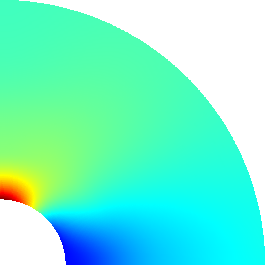
\includegraphics[width=.4\linewidth]{s_stress_contour} & 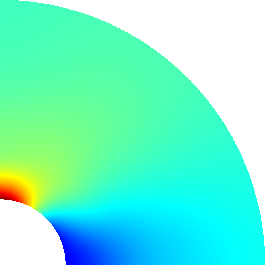
\includegraphics[width=.4\linewidth]{ns_stress_contour}\\
    $S-\mathcal{T}^{p} Q_4/Q_3$ & $NS-\mathcal{T}^{p} Q_4/Q_3$\\
    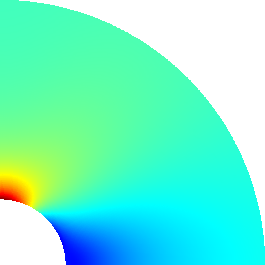
\includegraphics[width=.4\linewidth]{reference_stress_contour} & \includegraphics[width=.14\linewidth]{legend}\\
    Reference & Legend
    \end{tabular}
        \caption{ Contour plots of $\sigma_{xx}^h$ for the plate with a circular hole ($p=4$, and the finest mesh is used). For reference the analytical solution is also plotted. }
        \label{fig:platewithhole_contour}
\end{figure}

\begin{figure}[htb!]
    \center
    \begin{tabular}{cc}
    \includegraphics[width=.44\linewidth]{no} & \includegraphics[width=.5\linewidth]{g}\\
    $Q_4$ & $\mathcal{T}^{L^2} Q_4/Q_3$\\
    \includegraphics[width=.5\linewidth]{s} & \includegraphics[width=.5\linewidth]{ns}\\
    $S-\mathcal{T}^{p} Q_4/Q_3$ & $NS-\mathcal{T}^{p} Q_4/Q_3$
    \end{tabular}
        \caption{Contour plots of $\vert{\sigma_{xx}-\sigma_{xx}^h}\vert$ for the plate with a circular hole ($p=4$, and the finest mesh is used).}
        \label{fig:platewithhole_error_contour}
\end{figure}

\section{Conclusions}
\label{sec:conclusion}

We have presented two B\'{e}zier $\bar{B}$ projection methods, which we have called symmetric and non-symmetric \Bezier $\bar{B}$ projection, as an approach to overcome locking phenomena in structural mechanics applications of isogeometric analysis. Each approach maintains the sparsity of the resulting linear system. The methods utilize B\'ezier extraction and projection, which makes it simple to implement them in an existing finite element framework and makes it applicable to any spline representation which can be written in \Bezier form. In contrast to global $\bar{B}$ methods, which produce dense stiffness matrices, the B\'ezier $\bar{B}$ approach results in a sparse stiffness matrix while still benefiting from higher-order convergence rates. {We have made the connection between the non-symmetric method and a mixed formulation and shown that, although this method does not strictly satisfy the inf-sup condition, it reduces constraints sufficiently to provide optimal convergence rates for the problems studied here.}

We have demonstrated the performance of the approach in the context of shear deformable beams (to alleviate transverse shear locking) and nearly incompressible elasticity problems (to alleviate volumetric locking). The proposed method reduces locking errors and achieves nearly optimal convergence rates { for the symmetric method and optimal rates for the non-symmetric method}. The cases where optimal rates were not achieved {when using the the symmetric formulation are a symptom of the fact that the symmetric formulation is not directly related to a variational principle}.

{The two methods presented here provide a choice between a formulation that results in a symmetric stiffness matrix but requires matrix operations at the global level and potentially less accuracy and a formulation that results in a non-symmetric stiffness matrix that can be assembled in the standard element routine approach and achieves optimal convergence rates. The trade-offs are between higher costs in assembly for the symmetric formulation versus potentially higher costs in solving a non-symmetric system. In either case, however, the cost is less than using the standard $\bar{B}$ formulation.}